\documentclass{memoria}


\begin{document}

\portada{Informe Entrega 1: Ingeniería de Requerimientos}{Gerson Aguirre Pavez\\Max Chacón Villanueva\\Daniel Gacitúa Vásquez\\Elías González Marincovic\\Nicolás Rozas Sepúlveda}{\textbf{Profesores:}\\Mauricio Marín Caihuán\\Rodrigo Vásquez Fernández\\\textbf{Ayudante:\\}José Orellana}{\today}


\indices

%Introducción (No se incluye en los capítulos del documento)
%-------------------------------------------------------------------------------------
\capitulonn{INTRODUCCIÓN.}

En esta era tecnológica, las redes sociales han formado parte de las relaciones interpersonales, donde se asimila una interacción persona a persona tanto o más natural que en el mundo real. Existen distintas aplicaciones web con distintas funcionalidades para fines específicos dependiendo de los gustos de las personas. Por ejemplo, “Twitter” ofrece una plataforma dinámica de publicaciones con pocos caracteres donde la gente puede expresarse o informarse; “Facebook” permite interactuar con los contactos de manera más amplia, permitiendo publicaciones más extensas, incluyendo fotos, videos, archivos, entre otros; en tanto “Vine” permite subir videos de corta duración para expresar sentimientos, emociones o estados de ánimo.

En esta ocasión, se presenta “BitPhoto”, una plataforma ágil y dinámica que permite a distintos usuarios (profesionales o amateur) cargar fotografías e interactuar entre sus contactos, permitiendo un rápido feedback en sus comentarios. Además, permite localizar de manera geográfica las fotografías cargadas y muestra la información técnica pertinente de cada una de las imágenes, todo esto de manera rápida y actualizada.

Como en todo proceso de desarrollo, se requiere de una planificación previa para organizar los puntos importantes que se deben tomar en cuenta para lograr un resultado exitoso. En un primer acercamiento, se debe conocer y entender las necesidades para buscar una posible solución y de esta manera modelar no solo una solución eficaz, sino también eficiente. En esta primera entrega, la ingeniería de requerimientos será parte fundamental para cumplir con lo anteriormente mencionado, formando la base del desarrollo del producto final.

Para entender las necesidades que se deben cubrir con el software que se desarrollará, se analizarán los requerimientos funcionales y no funcionales, con los cuales se tendrá una idea general de las soluciones que deben plantearse. Posteriormente, se deben asimilar todas estas ideas para comenzar un modelamiento del problema, para esto, se utilizará el modelo de casos de uso y diagrama de clases de análisis, permitiendo una visualización un tanto más concreta de la información obtenida anteriormente.

Luego, en lo que se considera una proyección de lo que será el producto final, se utilizarán los prototipos de la interfaz de usuario, donde se observarán los bocetos de la aplicación web y cómo el usuario va a interactuar con ésta, además de un diseño conceptual de la base de datos para garantizar un funcionamiento óptimo del producto.
 
Todo lo anterior se deberá realizar en un ambiente de trabajo colaborativo del equipo, por lo que se definirán roles de los integrantes y las tareas que éstos deberán realizar. Para que exista una organización y coherencia entre quienes realizan las tareas, es que se trabajará con “Git”, un sistema de control de versiones en el cual se puede observar el trabajo que va haciendo cada integrante del equipo y revisarlo para dar una retroalimentación. Por lo mismo, es importante planificar una estimación de los tiempos en los que se tienen que hacer las distintas tareas y tener un registro para observar el cumplimiento de los deberes y analizar el avance del proyecto en general. Todo lo anterior se realizará con “Trello”, una plataforma interactiva y de fácil usabilidad para el equipo de trabajo, que asemejándose a una carta Gantt, mostrará si el avance en las distintas tareas va de acuerdo a lo propuesto o no.

Con esta entrega se espera tener resuelta la ingeniería de requerimientos, que es quizás, la fase más importante al momento de realizar un proyecto, puesto que constituye la base en la que se trabajará para implementar el resultado final. Con las correcciones que se harán con posterioridad, se comenzará la siguiente fase donde se trabajará la arquitectura para, de esta manera, comenzar a concretar las tareas realizadas en esta oportunidad.   



%-------------------------------------------------------------------------------------
\capitulo{MARCO TEÓRICO.}

\seccion{BASE DE DATOS RELACIONAL.}

Para mayor entendimiento, se define qué es un modelo relacional, el cual es uno de los más empleados a la hora de realizar una base datos. Éste es un tipo de modelo donde se puede generar relaciones entre tablas, las que son nombradas como entidades y éstas, a su vez, poseen ciertos atributos, los que poseen una conexión que se logra a través de las relaciones, para obtener la mayor información posible de la base de datos.\\

\seccion{DIAGRAMA DE CASOS DE USO.}

Antes de pasar a definir lo que es un diagrama de casos de usos, se debe comprender qué es un caso de uso, el cual puede ser considerado como una receta, debido a que entrega la descripción de los pasos a seguir, también muchas veces mencionado como un camino feliz a lo que se desea realizar. Además en un caso de uso se deben manejar ciertas excepciones que pueden ser producidas durante el seguimiento de los ya mencionados pasos.

Luego de ya entender lo que es un caso de uso, se procede a realizar la descripción de qué es un diagrama de casos de usos. Se debe partir por definir que este diagrama es de comportamiento UML, en este diagrama se deben definir los actores y casos de usos, donde se relacionan entre sí, para dar a entender la idea de que un actor realizará cierto caso de uso, es decir, este último es considerado una actividad a realizar por cierto actor. Para mayor entendimiento se muestra a continuación como debe ser un diagrama de casos de uso:\\

\figura{Ejemplo relación Actores/Casos de Uso}{
	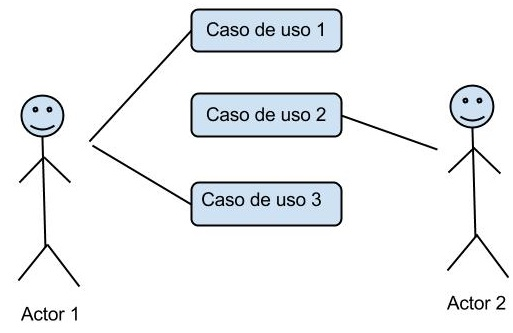
\includegraphics[width=10cm]{MarcoTeorico.jpg}
}


 
\seccion{DIAGRAMA DE CLASES.}

Es un diagrama que describe un sistema a crear, definiendo qué clases contendrá y que atributos tendrá cada una de estas, es decir, la idea de la creación de un diagrama de clases, es lograr entender de manera ordenada el sistema a crear y así no llegar y programar de manera desordenada, sino que sabiendo de cierta manera cómo será estructurado el sistema a crear.\\

\seccion{INGENIERÍA DE REQUERIMIENTOS.}

Esta comprende todas las tareas relacionadas con la determinación de las necesidades o de las condiciones a satisfacer para el software a realizar o reconfigurar, tomando en cuenta los requisitos que se relacionan al software correspondiente, esto sea realiza entre las partes interesadas, las que pueden entrar en conflicto entre ellos.\\

\seccion{REQUERIMIENTOS FUNCIONALES.}

Este tipo de requerimiento define una funcionalidad del software a realizar o de sus componentes, es decir, establecen el comportamiento del sistema y de qué manera el usuario interactúa con el mismo. En palabras simples, son todas las funcionalidades con las que el usuario se encuentra. Para describir estos requerimientos se recomienda empezar con "el usuario puede".\\

\seccion{REQUERIMIENTOS NO FUNCIONALES.}

Los requerimientos no funcionales, son requisitos que especifican ciertos criterios que pueden usarse para juzgar la operación de un sistema en lugar de sus comportamientos específicos. Estos requerimientos muestran cómo el sistema debe sostener y mantener la aplicación para su correcto funcionamiento. Para la descripción de estos requerimientos, se recomienda empezar con "el sistema debe".

%-------------------------------------------------------------------------------------
\capitulo{ENUNCIADO DEL PROBLEMA.}

Para el proyecto se pide replicar la red social “Flickr”. El principal objetivo de esta red social, es compartir las fotos de los usuarios y fomentar la retroalimentación mediante las interacciones que la aplicación permite.

Para realizar este trabajo se piden replicar ciertas funcionalidades de las distintas vistas que tiene “Flickr”. Las vistas y funcionalidades que se piden son las siguientes:

\begin{itemize}
    \item Vista perfil de usuario: Camera roll, Photo stream, Albums, Map, Favorities y Recent activities.
    \item Vista de personas: Photo from y Photo of.
    \item Vista explorar: Recemt potos, World map y Camera finder.
    \item Vista de búsqueda: Sort, Search y License.
    \item Vista subir imágenes: Add, Remove, Change name, Add tags, Add, people, Add to albums y Owner settings.
\end{itemize}

Para la realización del proyecto se pide conocer y desarrollar el problema con las siguientes tecnologías:

\begin{itemize}
    \item HTML5 en conjunto con AngularJS y jQuery.
    \item JavaEE y servicios del tipo RESTful.
    \item Sistema Operativo Móvil Android.
    \item MySQL Community Edition.
    \item Apache Lucene.
    \item Glassfish.
    \item Gradle.
    \item Weka.
    \item Git.
    \item Trello.
\end{itemize}

Para la presente entrega se contempla la etapa de ingeniería de requerimientos. Esta consta de todas las tareas que se deben determinar para tener claras las necesidades y condiciones para satisfacer el software que se desarrollará, en este caso la réplica de la red social “Flickr”. Esta entrega comprende el listado de requerimientos funcionales, que constan las funcionalidades especificas que debe tener el software y sus componentes y describen el comportamiento del sistema, además de la lista de requerimientos no funcionales, estos son los requisitos que no describen comportamientos o funciones, estos se enfocan en los detalles y características que debe poseer el sistema para su correcto funcionamiento.

Esta entrega también comprende el análisis de los casos de uso, en donde se listan y se describen los pasos para que se lleven a cabo los distintos procesos del software, e identificando los actores involucrados en los distintos procesos. Así también se debe presentar el modelo de casos de uso correspondiente, en donde se identifican los actores y se relacionan con los distintos casos de uso que el sistema debe satisfacer.

También se debe estudiar el diagrama de clases pertinente al problema, el cual describe la estructura de las distintas clases involucradas en el sistema y las relaciones que unen a éstas, también se deben presentar los métodos que contienen cada una de estas clases.

Para detallar el funcionamiento del sistema se pide un prototipo de interfaz de las diferentes vistas pedidas anteriormente, en donde se deben mostrar una vista previa de cada una de las vistas de la aplicación, detallando su funcionamiento y su diseño, además de nombrar las tecnologías que se ocuparon para la realización de éstas.

La presente entrega también comprende el diseño conceptual de la base de datos que se utilizará a futuro en la implementación del proyecto. Este modelo debe mostrar las distintas entidades que se identifican en el problema y las relaciones que se encuentran entre las distintas entidades. Para esto también se deben definir la cardinalidad de las relaciones para conocer el número de esta entidad que se puede generar en cada relación.

Para el fin de la primera etapa se pide realizar la definición de los distintos roles involucrados en la implementación del programa a realizar. El grupo debe definir los expertos en las distintas tecnologías que se exigen para la correcta realización del software, estos roles deben ser aceptados con responsabilidad por cada uno de los integrantes del grupo, ya que cada parte es fundamental para la correcta realización de las etapas de implementación y esencial para la finalización de este proyecto.

En resumen la ingeniería de requerimientos es la etapa base del proyecto, además es una etapa muy importante ya que se deben definir los límites y funcionalidades de las distintas partes de éste. Para la futura realización de estas funcionalidades se deben definir de manera correcta los requisitos funcionales y no funcionales, además de los distintos diagramas, ya que las entregas posteriores se deben basar en esta primera etapa para su correcta realización, implementación y funcionamiento.


%-------------------------------------------------------------------------------------
\capitulo{OBJETIVOS.}

\seccion{DE LA ASIGNATURA.}
\begin{enumerate}
	\item Profundizar en el uso de tecnologías de Bases de Datos Relacionales.
	\item Utilizar metodologías de desarrollo de software para concretar un proyecto a gran escala.
	\item Relacionarse con metodologías de desarrollo ágil (como Scrum).
\end{enumerate}


\seccion{DE INGENIERÍA DE REQUISITOS.}
\begin{enumerate}
	\item Lograr identificar los requisitos funcionales y no funcionales para el desarrollo óptimo de la aplicación.
	\item Identificar los actores del sistema. 
	\item Realizar un modelo de base de datos consistente, que sea capaz de responder a las necesidades de la aplicación. Con capacidad de soportar los requerimientos cambiantes.
	\item Realizar un prototipo de interfaz no desechable que sirva como base para las creaciones posteriores.
	\item Determinar cuales son los atributos propios de la API de flickr a utilizar y cuáles serán los nuevos.
\end{enumerate}

\seccion{DE COORDINACIÓN DE TRABAJO.}
\begin{enumerate}
	\item Lograr coordinar al grupo de trabajo para trabajar de manera óptima con la metodología especificada.
	\item Lograr asignar tareas de forma equitativa.
	\item Utilizar de manera eficiente los recursos y medios de comunicación para la coordinación del trabajo en equipo.
\end{enumerate}


%-------------------------------------------------------------------------------------
\capitulo{MISIÓN Y VISIÓN DEL PRODUCTO DE SOFTWARE.}

\seccion{MISIÓN.}

Nuestra misión como "Threads \& Bits Desarrolladores", organización destinada al desarrollo de aplicaciones web y móviles, es  lograr que las personas puedan compartir y hacer del mundo un lugar más abierto y conectado, ofreciendo a nuestros clientes productos de excelencia y con altos estándares de calidad cumpliendo así con sus expectativas y necesidades. Además, consideramos que nuestros clientes son de gran importancia para la organización, por lo cual, nos hemos propuesto entregar productos innovadores, que otorguen soluciones efectivas, seguras, confiables y de alta calidad para responder a las necesidades cambiantes, y contribuir así, a los objetivos particulares de cada uno de éstos, proporcionando de esta manera altos niveles de satisfacción.

Como organización creemos que “BitPhoto” será un producto que cumpla con las expectativas de nuestros clientes, con nuestra aplicación buscamos otorgar una nueva experiencia a las personas, queremos que las personas compartan sus fotografías, sus trabajos, su arte con el mundo, todo esto de manera cómoda, segura y confiable. El ideal de “BitPhoto” es que el usuario tenga la posibilidad de conectarse y comunicarse con todo el mundo, desde amigos o familiares hasta compañeros de trabajo. En conclusión en "Threads \& Bits Desarrolladores" queremos que "Bitphoto" se transforme en la red social, para fotógrafos amateurs y profesionales de más éxito a nivel nacional e internacional.\\


\seccion{VISIÓN.}

Ser una organización multidisciplinaria con el fin de ofrecer soluciones en diversas áreas, integrando la tecnología y principalmente la informática a éstas. Queremos ser una organización que genere confianza en nuestros clientes, y con la sociedad. Que la organización se caracterice por ser una fuente de inversión para el capital humano, permitiéndonos así crear productos de mejor calidad.

A futuro nos vemos como una organización de prestigio y seriedad en el mercado tanto nacional como internacional, logrando así con el tiempo, posicionarnos como un referente nacional en el desarrollo de soluciones informáticas para diversas áreas y campos de la sociedad actual. Queremos llegar a ser un motor que potencie el desarrollo de aplicaciones en nuestro país y latinoamérica, con alta presencia en el mercado internacional, mediante la utilización de tecnología de punta para la creación de nuestros productos. La visión a mediano o largo plazo es poder captar y cautivar a una amplia variedad de clientes, satisfaciendo sus necesidades de manera íntegra y efectiva. Buscamos trabajar con las grandes, medianas y pequeñas empresas en la implementación de soluciones vanguardistas que satisfagan sus necesidades.

"Threads \& Bits Desarrolladores" tiene como objetivo a corto plazo satisfacer el mercado nacional con la creaciones de nuestro producto “BitPhoto” el cual creemos que nos permitirá crecer y mejorar de manera continua, permitiéndonos de esta manera ampliar el mercado en el cual nos movemos  y mejorar la calidad de los servicios que ofrecemos a nuestros clientes.

Creemos que “BitPhoto” se transformará en la plataforma donde cada fotógrafo profesional o amateur podrá mostrar su trabajo al mundo y conectarse más por medio de las redes sociales.  También tenemos la visión que “BitPhoto” permitirá a organizaciones de distintas índoles mostrar sus actividades por medio de la fotografía. Y creemos firmemente que “BitPhoto” se transformará en la aplicación más utilizada por las personas para almacenar y compartir sus fotografías con familia, amigos, compañeros de trabajo, entre otros.


%-------------------------------------------------------------------------------------
\capitulo{REQUERIMIENTOS DEL SISTEMA.}

\seccion{REQUERIMIENTOS FUNCIONALES.}

\subseccion{VISTA PERFIL DE USUARIO.}

\textbf{- Camera Roll:}

RF1: El usuario puede ver las fotografías organizadas por fecha, escogiendo por la fecha en que fueron tomadas o la fecha en que fueron cargadas a la aplicación.\\

\textbf{- Photo stream:}

RF2: El usuario puede visualizar las fotografías que ha cargado sin importar si éstas se encuentran en álbumes distintos.

RF3: El usuario puede seleccionar una fotografía cargada para revisar en detalle los datos importantes de ésta (etiquetas, personas que se encuentran en la foto, comentarios, datos técnicos de la cámara, lugar, fecha, cuantas veces ha sido vista y cuantas personas han marcado como favorita la fotografía).

RF4: El usuario puede agregar personas en una fotografía cargada.

RF5: El usuario puede agregar tags o etiquetas a una fotografía cargada.

RF6: El usuario puede comentar una fotografía cargada.

RF7: El usuario puede agregar o mover una fotografía de un álbum a otro.\\

\textbf{- Albums:}

RF8: El usuario puede visualizar los distintos álbumes creados con una de las fotografías que contengan como carátula.

RF9: El usuario puede seleccionar un álbum para visualizar todas las fotografías contenidas en éste.

RF10: El usuario puede crear un nuevo álbum ingresando datos importantes como un nombre, una descripción, y una o más fotografías que ya se encuentren cargadas en la aplicación. \\

\textbf{- Map:}

RF11: El usuario visualiza un mapa del mundo donde puede ubicar de manera geográfica las fotografías que ha cargado, guardándose una dirección donde puede observar la fotografía. 

RF12: El usuario puede buscar una dirección en el mapa. \\

\textbf{- Favorites:}

RF13: El usuario puede visualizar las fotografías de otras personas donde ha marcado la opción “favorito”.\\\\\\

\textbf{- Recent Activity:}

RF14: El usuario puede ver las últimas interacciones relacionadas con actividad en sus fotos, respuestas a sus comentarios en fotos de otras cuentas, notificaciones de seguimiento (follow y followback) y fotos en las que se ha añadido.

RF15: El usuario puede seleccionar un período de tiempo para ver las interacciones que ocurrieron.\\

\subseccion{VISTA DE PERSONAS.}

\textbf{- Photos from:} 

RF16: El usuario puede  ver entre 1 o 5 fotos de las personas a los cuales está siguiendo.\\

\textbf{- Photo of:} 

RF17: El usuario puede visualizar las fotografías en las que se han marcado personas a las que está siguiendo.\\

\subseccion{VISTA EXPLORAR.}

\textbf{- Recent photos:}

RF18: El usuario puede visualizar las fotos recientemente subidas a la aplicación sin importar si sigue o no a las demás personas.

RF19: El usuario puede marcar la opción “favorito” en cualquiera de las fotografías recientes.

RF20: El usuario puede comentar cualquiera de las fotografías recientes.

RF21: El usuario puede ver toda la información técnica de las fotografías recientes.\\

\textbf{- World Map:}

RF22: El usuario puede ver el mapa mundial de fotografías que han sido subidas con ubicación a la aplicación sin importar si está siguiendo o no a las personas.

RF23: El usuario puede seleccionar una marca en el mapa de un lugar específico (país o ciudad) para ver las fotografías localizadas en esa ubicación.

RF24: El usuario puede buscar una dirección, un país o una ciudad  en el mapa, para visualizar todas las fotografías que se han marcado en dicho lugar.\\

\textbf{- Camera Finder:}

RF25: El usuario puede ver las cámaras más populares con las que se han tomado fotografías subidas a la aplicación.

RF26: El usuario puede ver un listado de las distintas marcas de cámaras que se han utilizado.

RF27: El usuario puede ver las especificaciones técnicas de las distintas cámaras, seleccionando un modelo en el listado de cámaras populares.

RF28: El usuario puede visualizar las fotografías que fueron sacadas con una cámara en específico.\\

\subseccion{VISTA DE BÚSQUEDA.}

\textbf{- Sort:} 

RF29: El usuario puede ordenar la búsqueda por orden de relevancia, fotografías recientes o fotografías interesantes.\\

\textbf{- Search:}

RF30: El usuario visualiza las fotografías relacionadas con las palabras clave de su búsqueda.

RF31: El usuario puede filtrar la búsqueda por las fotografías de todos, por sus propias fotografías, por fotografías de sus contactos o usuarios.\\

\textbf{- License:}

RF32: El usuario puede filtrar la búsqueda, mostrándose solo fotografías con permiso comercial, con permiso de modificación, con ambos permisos o fotografías con cualquier tipo de licencias.\\

\subseccion{VISTA SUBIR IMÁGENES.}

\textbf{- Add:}

RF33: El usuario puede arrastrar una o varias fotografías o buscarlas en los directorios de su equipo para cargarla a la aplicación.\\

\textbf{- Remove:} 

RF34: El usuario puede remover una o varias fotografías que hayan sido seleccionadas para ser cargadas a la aplicación.\\ 

\textbf{- Change name:}

RF35: El usuario puede cambiar el nombre de una o varias fotografías que hayan sido seleccionadas para ser cargadas a la aplicación.\\

\textbf{- Add tags:}

RF36: El usuario puede agregar variadas etiquetas o tags a una o varias fotografías que hayan sido seleccionadas para ser cargadas a la aplicación.\\

\textbf{- Add people:}

RF37: El usuario puede agregar distintas personas en una o varias fotografías que hayan sido seleccionadas para ser cargadas a la aplicación.\\

\textbf{- Add to albums:}

RF38: El usuario puede agregar una o varias fotografías, que hayan sido seleccionadas para ser cargadas a la aplicación, a distintos álbumes sin importar si estos ya ha existen o deben crearse.\\

\textbf{- Owner Settings:}

RF39: El usuario puede escoger la licencia que desee para una o varias fotografías que hayan sido seleccionadas para ser cargadas a la aplicación.\\

\subseccion{VISTA INICIAR SESIÓN.}

RF40: El usuario puede ingresar sus datos de registro para iniciar sesión.\\

\newpage

\seccion{REQUERIMIENTOS NO FUNCIONALES.} 

RNF1: La aplicación deberá estar disponible para teléfonos móviles con sistema operativo Android (4.0 IceCream Sandwich de Android o superior).

RNF2: La aplicación Web debe usar la tecnología AngularJS.

RNF3: La forma de persistir la información del sistema será mediante una base de datos relacional ocupando el gestor de base de datos MySQL.

RNF4: La base de datos debe ofrecer soporte a datos geoespaciales con formato WKT (Well-Known Text).

RNF5: El sitio web del sistema debe utilizar HTML5 para sus vistas.

RNF6: El sistema debe someter a análisis los comentarios de los usuarios del sistema, con el fin de analizar sentimientos (positivo,negativo,neutral) mediante la herramienta Weka.

RNF7: El sistema debe implementar un motor de búsqueda mediante la indexación de tags y comentarios, utilizando la  herramienta APACHE Lucene.

RNF8: El sistema debe permitir geolocalizar fotografías.

RNF9: El sistema debe utilizar JavaEE para la creación del web service de tipo RESTful.

RNF10: La aplicación tanto web como móvil tendrá su interfaz en español latino.

RNF11: La aplicación debe poseer un diseño web adaptativo (\textsl{Responsive Web Design}).

RNF12: La aplicación web debe desplegarse en los navegadores web Chrome (versión 35 o superior), Firefox (versión 30 o superior), Opera (versión 20 o superior), Safari (versión 7 o superior), Internet Explorer (versión 9 superior).

RNF13: La base de datos del sistema debe ser alimentada por medio de la API de Flickr.

RNF14: El sistema debe velar por la privacidad de sus usuarios, el sistema no puede divulgar información que los usuarios no han autorizado.

RNF15: La aplicación Web y Móvil debe permitir identificar en todas sus vistas el nombre o icono de “BitPhoto”.

RNF16: La aplicación web y móvil debe indicar al usuario en qué instancia se encuentra.

RNF17: La aplicación web y móvil deberá estar habilitada 24 horas al día y los 7 días de la semana de manera regular.

RNF18: La aplicación se debe desarrollar utilizando el lenguaje de programación Java con algunas características de la versión JEE con las tecnologías CDI, JPA, EJB, JAX-RS.

RNF19: El servidor de aplicaciones que el sistema debe usar es GlassFish.

RNF20: El sistema debe señalar errores de la aplicación o de ejecución al usuario.

RNF21: En caso de falla de un componente del sistema no debe haber pérdida de información.

RNF22: El sistema entregará información actualizada de los usuarios y sus imágenes en  el sistema.

RNF23: Los formatos de fotografías permitidos por la aplicación serán JPEG y PNG no animado.

RNF24: La cantidad de fotografías soportadas por álbumes en el sistema será de 20 fotos.

RNF25: La aplicación tanto web como móvil deben señalar al usuario las condiciones de privacidad y uso de datos del usuario.

RNF26: La aplicación web debe indicar al usuario que componentes del dispositivo se utilizarán para la aplicación, y debe solicitar permiso para su uso.

%-------------------------------------------------------------------------------------
\capitulo{CASOS DE USO.} 

\seccion{LISTADO DE CASOS DE USO.}

Los casos de uso que se pueden identificar a partir de los requerimientos funcionales y de las funcionalidades que requiere el sistema, son los siguientes:

\begin{enumerate}
    \item Revisando historial de fotografías cargadas.
    \item Revisando fotografías cargadas.
    \item Revisando álbumes creados.
    \item Visualizando mapa de fotografías cargadas.
    \item Editando localización de fotografías cargadas.
    \item Visualizando fotos marcadas como favoritos.
    \item Visualizando actividad reciente de otros usuarios.
    \item Visualizando fotos de usuarios a quienes se está siguiendo.
    \item Visualizando fotografías en las que se han marcado personas a las que se está siguiendo.
    \item Visualizando fotografías recientemente cargadas a la aplicación.
    \item Visualizando mapa mundial de fotografías cargadas.
    \item Visualizando cámaras que se han utilizado con la aplicación.
    \item Buscando palabras clave.
    \item Subiendo imágenes.
    \item Interactuando con fotografías cargadas.
\end{enumerate}
\newpage

\seccion{DIAGRAMA DE CASOS DE USO.}

Se ha identificado solamente un actor que interactúa con el sistema utilizando las funcionalidades que se han especificado anteriormente. El usuario de la aplicación se ha denominado "Usuario BitPhoto", y el modelo de casos de uso se presenta a continuación:\\

\figura{Diagrama de Casos de Uso (completo)}{
	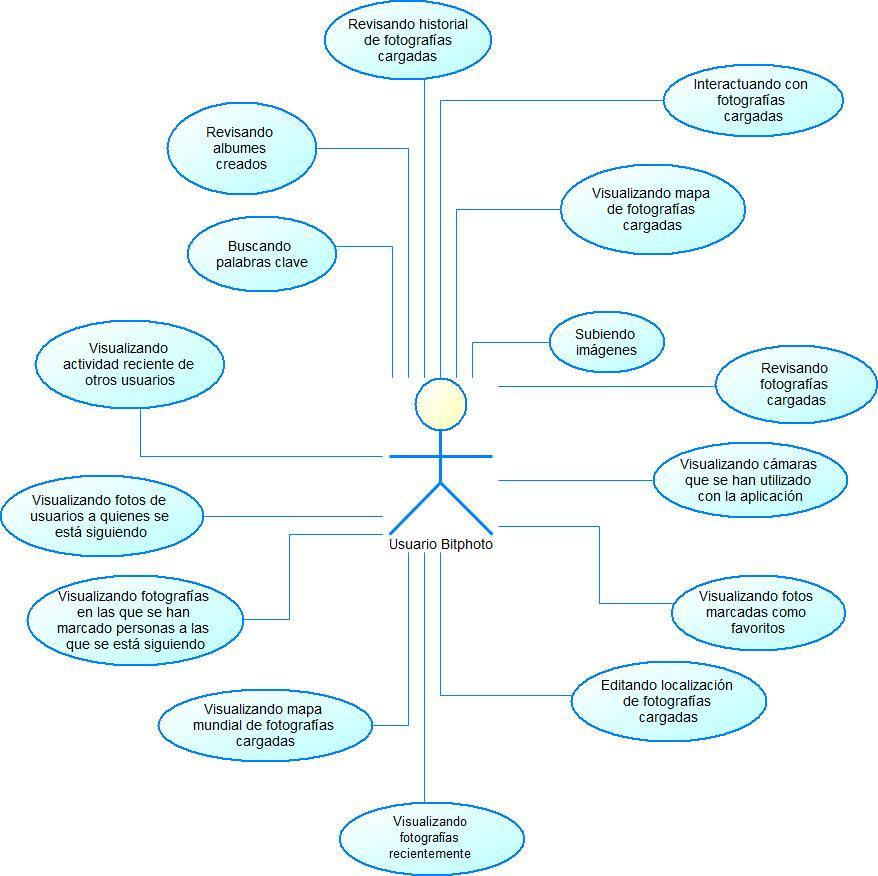
\includegraphics[width=15cm]{DiagramaDeCasosDeUso.jpg}
}

%-------------------------------------------------------------------------------------
\capitulo{MODELO DE CLASES DE ANÁLISIS.}

\seccion{DIAGRAMA DE CLASES.}

\figura{Diagrama de Clases (completo)}{
	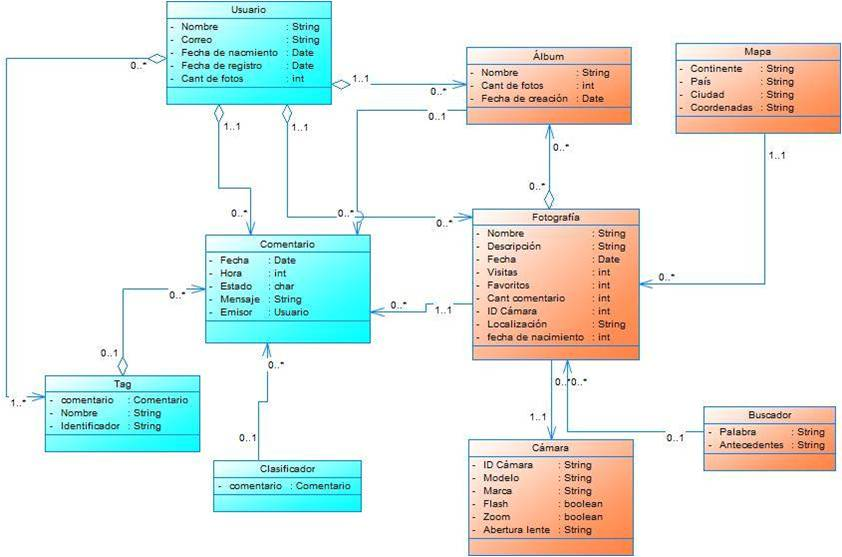
\includegraphics[width=15cm]{DiagramaDeClases.jpg}
}

Como se puede apreciar en la imagen anterior, el diagrama de clases consta de nueve clases necesarias para la implementación de la aplicación, las cuales serán explicadas a continuación:

\begin{itemize}
    \item \textbf{Usuario}: Debido a que la aplicación será utilizada por usuarios, los cuales poseerán una cuenta para la identificación de éste, es por eso que deberá contener los atributos necesarios. 
    \item \textbf{Álbum}: Ya que la aplicación contendrá imágenes, estás podrán ser almacenadas en álbumes, donde en el cual tendrá un nombre, cierta cantidad de fotos y la fecha de creación. (solo si es necesario implementarlo).
    \item \textbf{Mapa}: Debido a que cada imagen tendrá una ubicación de subida, es posible ubicarla dentro de un mapa.
    \item \textbf{Comentario}: Cada imagen en la aplicación podrá tener comentarios que pueden ser hechos por la misma persona que la subió o por alguna persona dentro de sus círculo de amigos, además estos serán clasificados en la escala positivo, negativo o neutral.
    \item \textbf{Fotografía}: Esta clase es la principal, debido a que es a lo que la aplicación está enfocada, estas podrán ser subidas en la aplicación por los distintos usuarios ya mencionados.
    \item \textbf{Tag}: En la aplicación será posible la utilización de ciertos tag a disposición de los usuarios, donde podrán ser utilizados para hacer referencia común en ciertas imágenes que los estos deseen.
    \item \textbf{Clasificador}: Como ya se menciona anteriormente los comentarios serán clasificados en una escala, esta clase será la encargada de realizar estas clasificaciones según un análisis del comentario realizado.
    \item \textbf{Cámara}: Dentro de la aplicación se maneja cierta información de las cámaras que han sacado ciertas fotos, esta clase será la encargada de extraer cierta información.
    \item \textbf{Buscador}: Entre las funcionalidades de la aplicación está la búsqueda de usuarios y fotos, esta clase es la encargada de que esta funcionalidad sea realizada.   
\end{itemize}


\newpage

Para mayor entendimiento en la explicación del diagrama se toma la decisión de dividir en dos partes éste, la parte celeste representando la gran clase Usuario y sus acompañantes, y la parte de color anaranjado en representación de la clase Fotografía y sus clases acompañantes:

\figura{Diagrama de Clases (sección 1)}{
	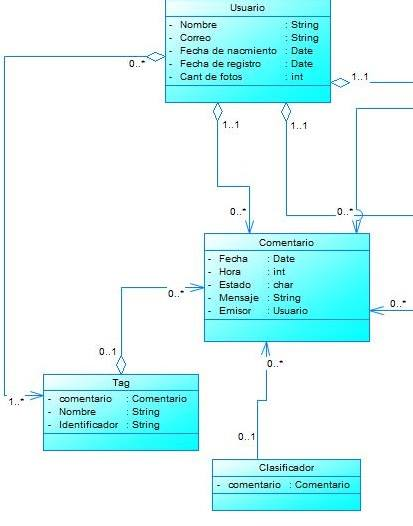
\includegraphics[width=14cm]{DiagramaDeClases2.jpg}
}

Como se puede apreciar la clase Usuario posee relación con Tag y clasificador, en significado de que un usuario puede realizar 1 o muchos tag en ciertos comentarios, esta relación quiere decir que el Tag necesita de la clase usuario para poder ser creados, es decir, como es usuario el que crea tag en el sistema se relacionan en agregación al igual que la relación entre comentario y usuario. 
Además se puede observar la clase clasificador, la cual representa una de las herramientas a implementar, la que tiene como finalidad otorgar de un estado a un comentario, el cual puede ser positivo, negativo o neutral, es por esto que clasificador posee como atributo un comentario.
Cabe mencionar que un usuario puede subir fotografias, que en fin esta es la primordial funcionalidad del sistema, además un usuario puede crear ciertos álbumes, donde puede suministrar de atributos a estos álbumes como a las fotografías.
Finalizando con esta parte también se puede destacar que existe una relación entre comentario y fotografía, la cual representa que una fotografía posee ciertos comentarios, los cuales pueden ser desde cero a muchos comentarios, los cuales pueden ser agregados por usuarios ajenos a la fotografía, así como el mismo usuario que la subió.

\figura{Diagrama de Clases (sección 2)}{
	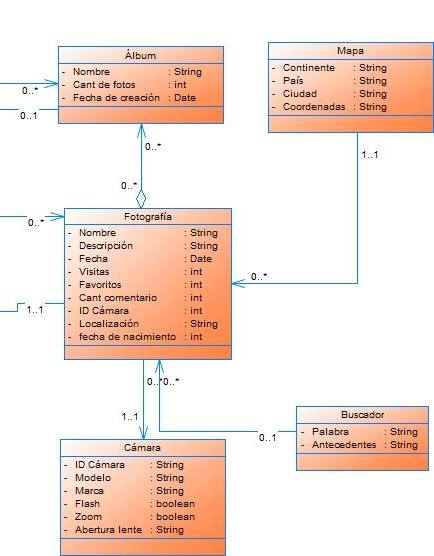
\includegraphics[width=14cm]{DiagramaDeClases3.jpg}
}

Siguiendo con la ya mencionada parte anterior, se puede apreciar que está la clase principal que es fotografía, primordial por el hecho de que el sistema está basado en el uso de las fotografías. Es acá donde se ve que un álbum posee ciertas fotografías, es decir, un álbum posee cero o muchas de estas fotografías.
La clase mapa está relacionada con la clase fotografía, debido a que la idea de esta clase es posicionar en un mapa mundial ciertas fotografías que se han cargado en ciertas ubicaciones dentro del mundo, Es así como se representa dentro de los atributos de la fotografía una localización, es por esta funcionalidad que sea decidido agregar una nueva clase llamada mapa.
Por otro lado se tiene la clase Buscador, la cual posee la funcionalidad de poder realizar una búsqueda con el ingreso de palabras claves y antecedentes dentro del sistema, esto con la idea de que se tiene en cuenta que el sistema funcionará para una gran cantidad de usuarios y se desea facilitar la tarea de encontrar ciertos aspectos en el sistema por parte del usuario.
Finalmente la clase Cámara, que está relacionada con la clase fotografía, esto debido a que se agrega como funcionalidad que el sistema pueda asociar la cámara que capturó la fotografía 


%-------------------------------------------------------------------------------------
\capitulo{BASE DE DATOS.}

A continuación se presenta el modelo conceptual de base de datos de la aplicación, con las entidades y relaciones entre estas, además se presentan el tipo de cardinalidad de la relación y en qué casos es mandatoria.

\figura{Modelo Conceptual base de datos con PowerDesigner v16.1}{
	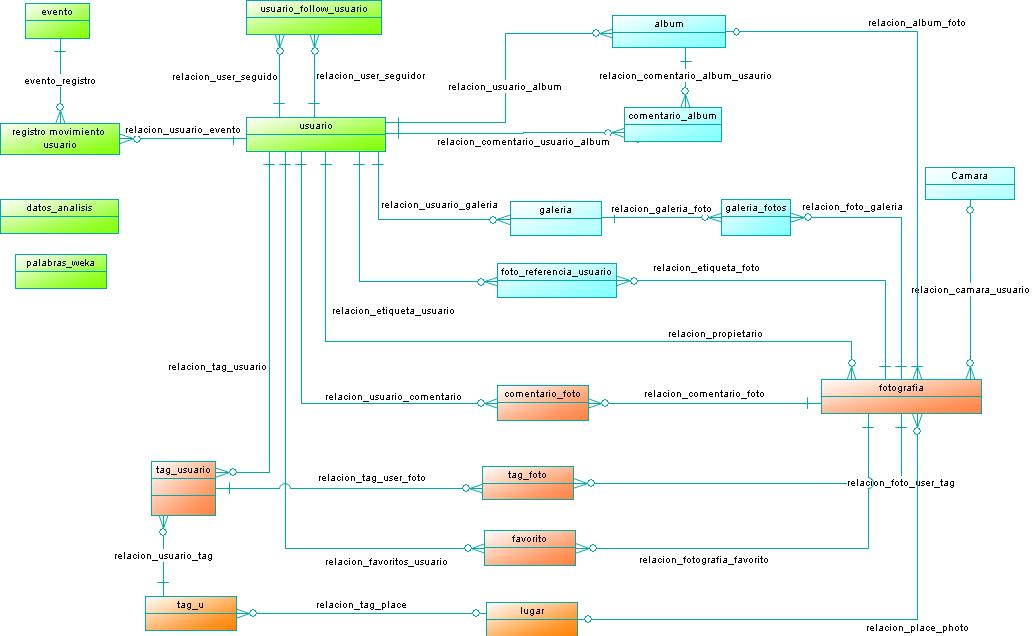
\includegraphics[width=15cm]{ImagenesMCDB/DiagramaConcBD.jpg}
}

\seccion{DESCRIPCIÓN DE TABLAS.}

\begin{itemize}
	\item evento: contiene información sobre los tipos de eventos que pueden realizar, o gatillar por parte del usuario en el sistema, por ejemplo borrar fotografia, seguir a otro usuario, comentar una foto, etc.
	\item registro\_movimiento\_usuario: contiene información sobre el evento en específico, asociado a un determinado usuario, fecha en que se realizó el evento, quien lo realizó, entre otras.
	\item datos\_analisis: contiene información de análisis respecto de la aplicación, número de personas que la utilizaron durante el dia, fotos subidas por dia, comentarios por dia, etc.
	\item usuario: contiene datos sobre el usuario de la aplicación, los permisos con los que cuenta su perfil, localización del usuario, nick de usuario, entre otros.
	usuario\_follow\_usuario: contiene datos sobre la relación entre seguido y seguidor, de manera unidireccional, también contendrá la fecha en que se realizó esta actividad.
	\item palabras\_weka: contiene información sobre cada palabra considerada para el desarrollo de la aplicación web, palabra, frecuencia utilizada, el peso relativo de la palabra, etc.
	\item album: contiene información sobre el álbum creado por determinado usuario.Descripción, fecha de creación, número de fotos en el álbum, etc.
	\item comentario\_album: contiene información sobre los comentarios realizados por los determinados usuarios a determinados álbumes.
	\item galeria: contiene datos sobre las galerías creadas por los usuarios de la aplicación.( Los atributos de esta tabla no están especificados ya que no se agregara esta funcionalidad al sistema, pero igual se agregó como tabla, para futuras implementaciones , como también para mostrar la modularidad del modelo, que permite agregar nuevas tablas).
	\item foto\_referencia\_usuario: contiene información sobre las personas que se encuentran en determinadas fotos, se indica la posición en la cual se encuentran dentro de la fotografia, la fotografia y el usuario al cual se hace referencia.
	\item galeria\_fotos: contiene información sobre la relación entre una foto y determinada galería (Al igual que para galería los atributos de esta tabla no se encuentran definidos en su totalidad por circunstancias similares).
	\item camara: contiene información sobre las cámaras utilizadas para la tomas de las fotos. datos como el modelo, características de zoom, cuantos MP posee, etc.
	\item tag\_u: contiene información sobre el tag que utilizan de manera generalizada los usuarios de la aplicación.
	\item fotografia: contiene información sobre las fotografías, contiene gran cantidad de atributos, y muchos de ellos puede que no se utilicen en primera instancia, por lo cual se agregaron todos los entregados por la API de Flickr.
	\item comentario\_foto:contiene información sobre los comentarios realizados por usuarios hacia ciertas fotografías, la fecha en que realizó el comentario, entre otras cosas. 
	\item tag\_usuario: contiene información sobre el tag y quien utilizó determinado tag.
	\item tag\_foto:contiene información sobre qué tags fueron utilizados para determinada fotografía.
	\item lugar: contiene información sobre los lugares a los cuales puede hacer referencia una fotografía.
	\item favorito: contiene información sobre la relación entre favoritos, cuando un usuario agrega una foto de otro usuario como favorita.
\end{itemize}

\newpage

\seccion{DESCRIPCIÓN DE RELACIONES.}

\figura{Modelo Conceptual Base de Datos (Parte 1)}{
	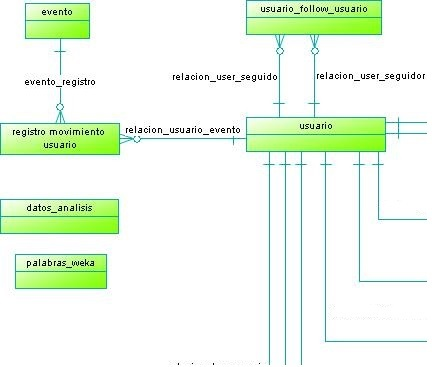
\includegraphics[width=15cm]{ImagenesMCDB/MBD1.jpg}
}

En la figura anterior se observa la relación que existe entre las entidades evento, registro\_ movimiento\_usuario, usuario y usuario\_follow\_usuario. Primero usuario\_follow\_usuario se relaciona con usuario mediante una asociación doble, lo cual hace referencia que un usuario puede ser seguido por otro usuario en el sistema, esta representación será unidireccional.
Esta parte de la base de datos permitirá respaldar la información sobre qué usuarios se encuentran siguiendo a otros.
Luego en la relación usuario y registro\_movimiento\_usuario se representa que un usuario puede tener registros de movimiento de usuario, y a su vez estos pueden ser por diversos tipos de eventos. Cabe señalar que en registro\_movimiento\_usuario y usuario\_follow\_usuario convergen en relaciones muchos a muchos por los cual ambas tablas al pasar del modelo conceptual al lógico tendrán identificadores de las tablas con las cuales se relacionan.


\figura{Modelo Conceptual Base de Datos (Parte 2)}{
	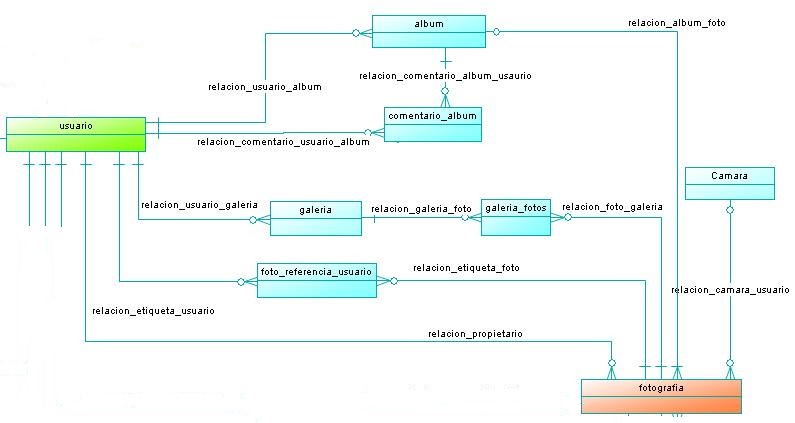
\includegraphics[width=15cm]{ImagenesMCDB/MBD2.jpg}
}

En la figura recién expuesta se presenta la relación entre las tablas usuario y fotografía entre las cuales se encuentran otras tablas como lo son, album, galeria, foto\_referencia\_usuario, comentario\_album. Además se presenta una tabla que solo se relaciona de manera directa con fotografía como lo es Camara. 
Primero mediante la relación propietario se relaciona fotografía con usuario, ya que un usuario puede poseer fotografías. En relación a la tabla foto\_referencia\_usuario, ésta se relaciona con usuario y fotografía convergiendo en una relación muchos a muchos. Tambien tenemos álbum pertenece un usuario, a su vez fotografía, pertenece a determinado álbum. 
La tabla comentario\_album es convergencia de una relación mucho a mucho entre usuario que comenta un álbum. 
Las entidades galeria y galeria\_fotos no se explicaran por el momento, hasta tener claro si se considerara o no esta funcionalidad. La tabla camara se relación con la tabla fotografía, ya que una fotografía puede ser tomada con una determinada cámara. 

\figura{Modelo Conceptual Base de Datos (Parte 3)}{
	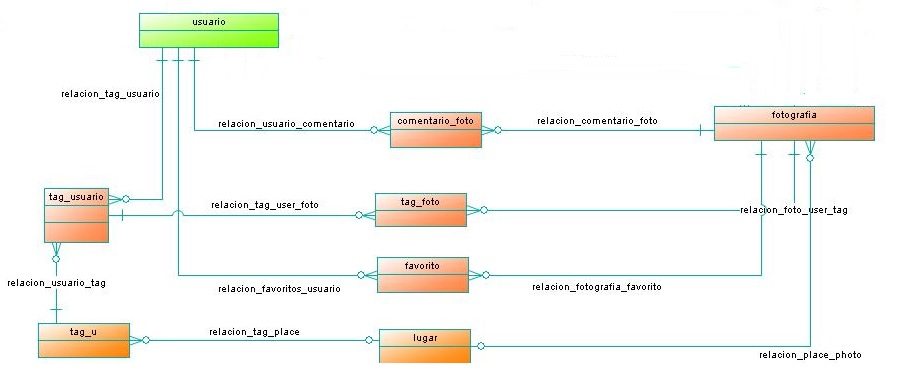
\includegraphics[width=15cm]{ImagenesMCDB/MBD3.jpg}
}

En la figura anterior Se presenta la relación que existe entre usuario y fotografía mediante las tablas comentario\_foto, tag\_foto, tag\_usuario, tag\_u, lugar y favorito. La tabla comentario\_foto se relaciona con el usuario que realizó el comentario y con la fotografía que se comento. A su vez la tabla favoritos se relaciona con la tabla usuario que tiene como favorita una determinada fotografía. Luego se presentan las tablas tag\_usuario que permitirá tener información sobre qué tag utiliza cada usuario y mediante tag\_foto determinar quien colocó determinado tag a una determinada fotografía. También se tendrá como dato el tag a nivel generalizado ya que muchos usuarios pueden utilizar el mismo tag. Los tag también hacen referencia a lugares por eso la relación entre tag\_u y lugares, esta relación permitirá mediante el buscador encontrar fotos que referencian lugares del mundo. Cabe señalar que dependiendo de la fotografía se tendrán datos o no respeto a su geolocalización y a su vez datos sobre el lugar en el cual fue tomada.


\seccion{ENUMERACIÓN DE ATRIBUTOS.}

A continuación se mostrarán las tablas con sus respectivos atributos, cabe destacar que puede que los atributos considerados no se utilicen en su totalidad y que pueden estar sujetos a cambios.

\figura{Atributos de Tablas (parte 1)}{
	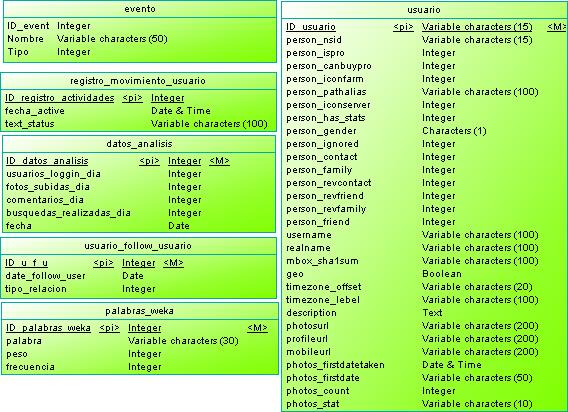
\includegraphics[width=15cm]{ImagenesMCDB/Tabla1.jpg}
}

\figura{Atributos de Tablas (parte 2)}{
	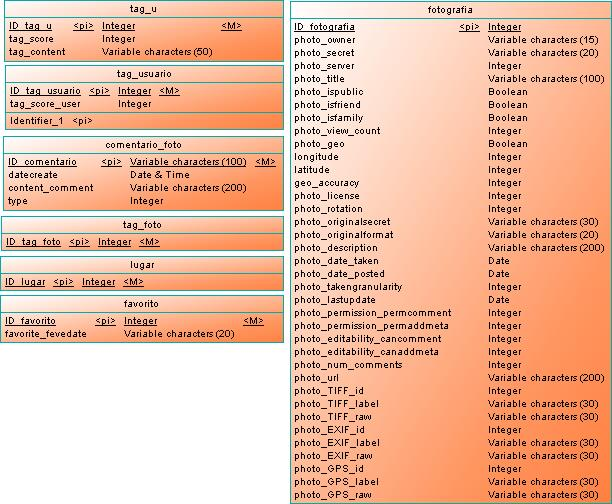
\includegraphics[width=15cm]{ImagenesMCDB/Tabla2.jpg}
}

\figura{Atributos de Tablas (parte 3)}{
	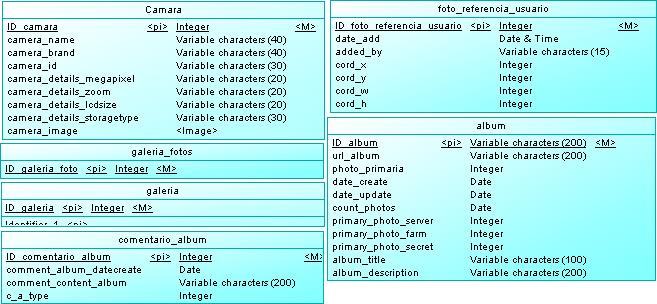
\includegraphics[width=15cm]{ImagenesMCDB/Tabla3.jpg}
}


%-------------------------------------------------------------------------------------
\capitulo{PROTOTIPO DE INTERFAZ DE USUARIO.}

Para tener una idea de la plataforma a desarrollar, se generó un Prototipo de Interfaz de Usuario que permitiese tener una idea de cómo luciría la interfaz web de la aplicación, y así recolectar información importante que ayudará a la etapa del diseño de la aplicación. A continuación se hará una descripiciónn breve de las vistas más relevantes, junto con una representación gráfica de éstas.

\seccion{VISTAS DE INICIO.}

En la vista de inicio se ve la peresntación sencilla de la web de BitPhoto, potenciada por HTML5 y estilizada con los elementos de Bootstrap.
\figura{Vista Inicio}{
	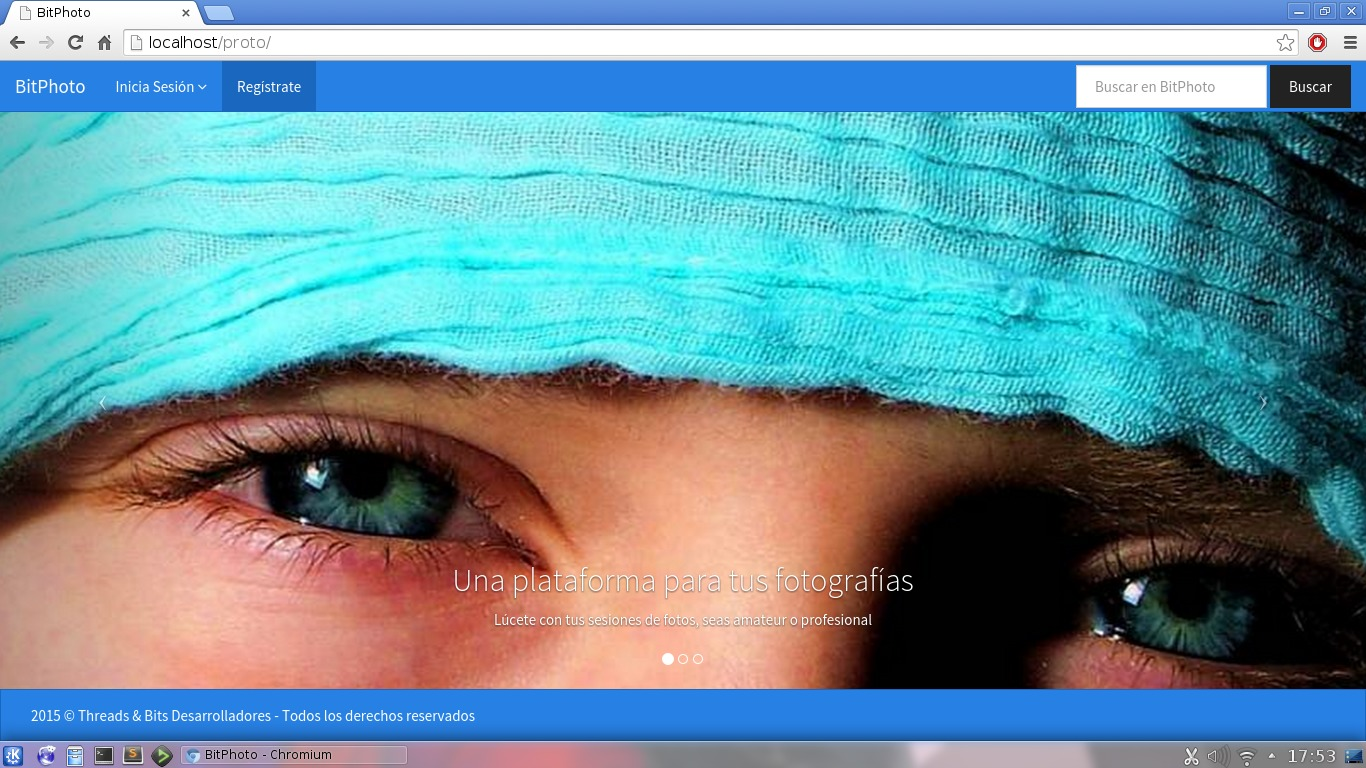
\includegraphics[width=14cm]{proto/01.jpg}
}

El formulario de registro muestra un estilo claro y sencillo.
\figura{Vista Registro}{
	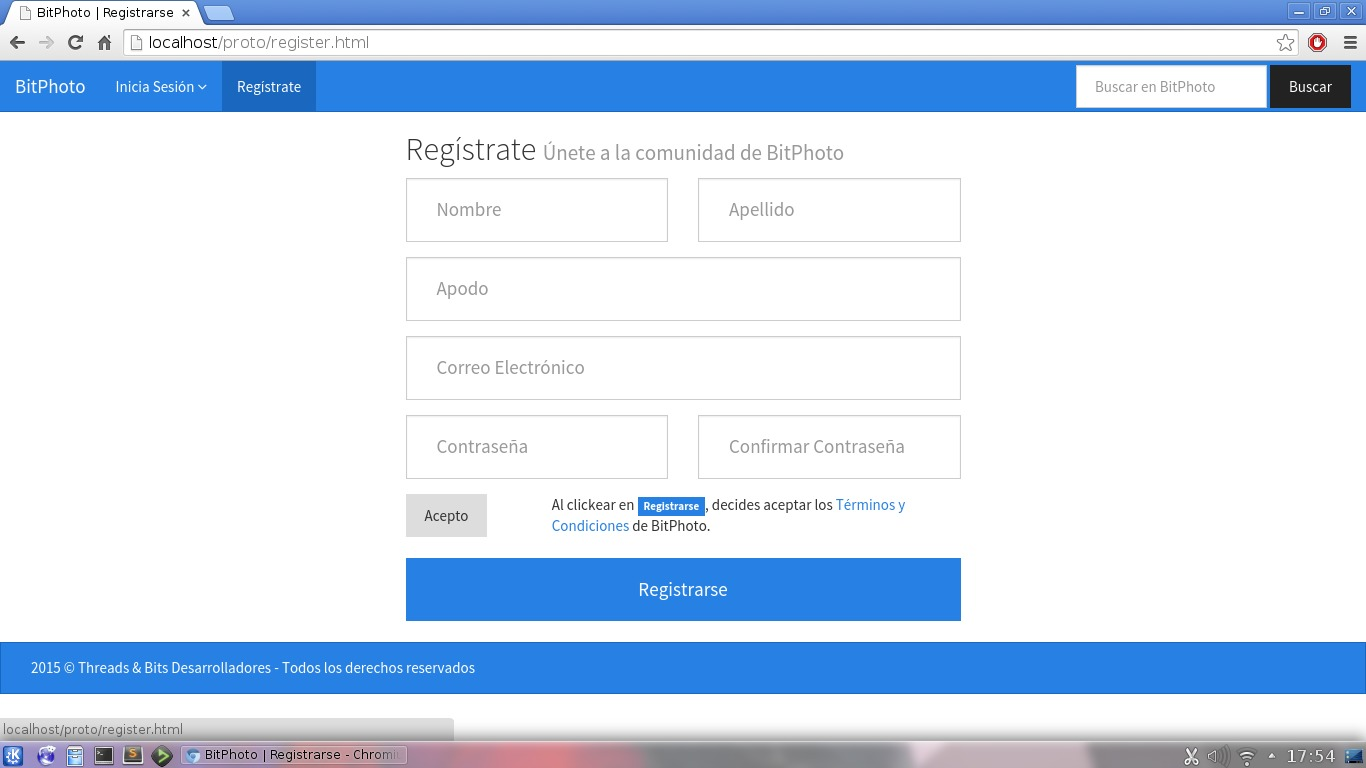
\includegraphics[width=14cm]{proto/02.jpg}
}

El formulario de acceso a la plataforma (login) se ha dispuesto como un submenú por claridad y agilidad de acceso.
\figura{Vista Login}{
	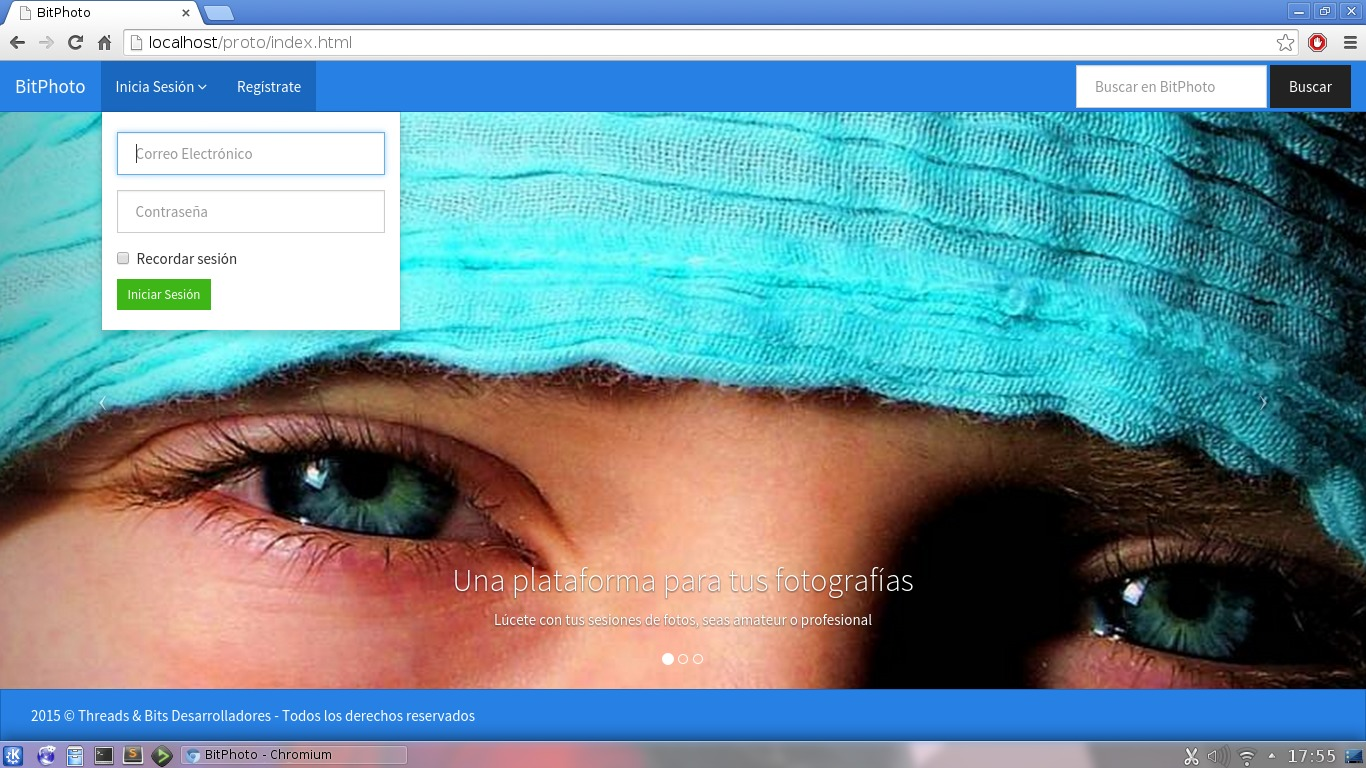
\includegraphics[width=14cm]{proto/03.jpg}
}

\newpage

\seccion{VISTAS DE USUARIO.}

La sección Home al hacer login en la plataforma muestra fotos destacadas de los usuarios de la plataforma, junto con información del sitio. Nótese que algunos elementos (como la cabecera y el pie de página) fueron diseñados como vistas HTML independientes, y son cargadas dentro de una vista base via jQuery (esto favorece la rapidez de edición de las vistas).
\figura{Vista Home}{
	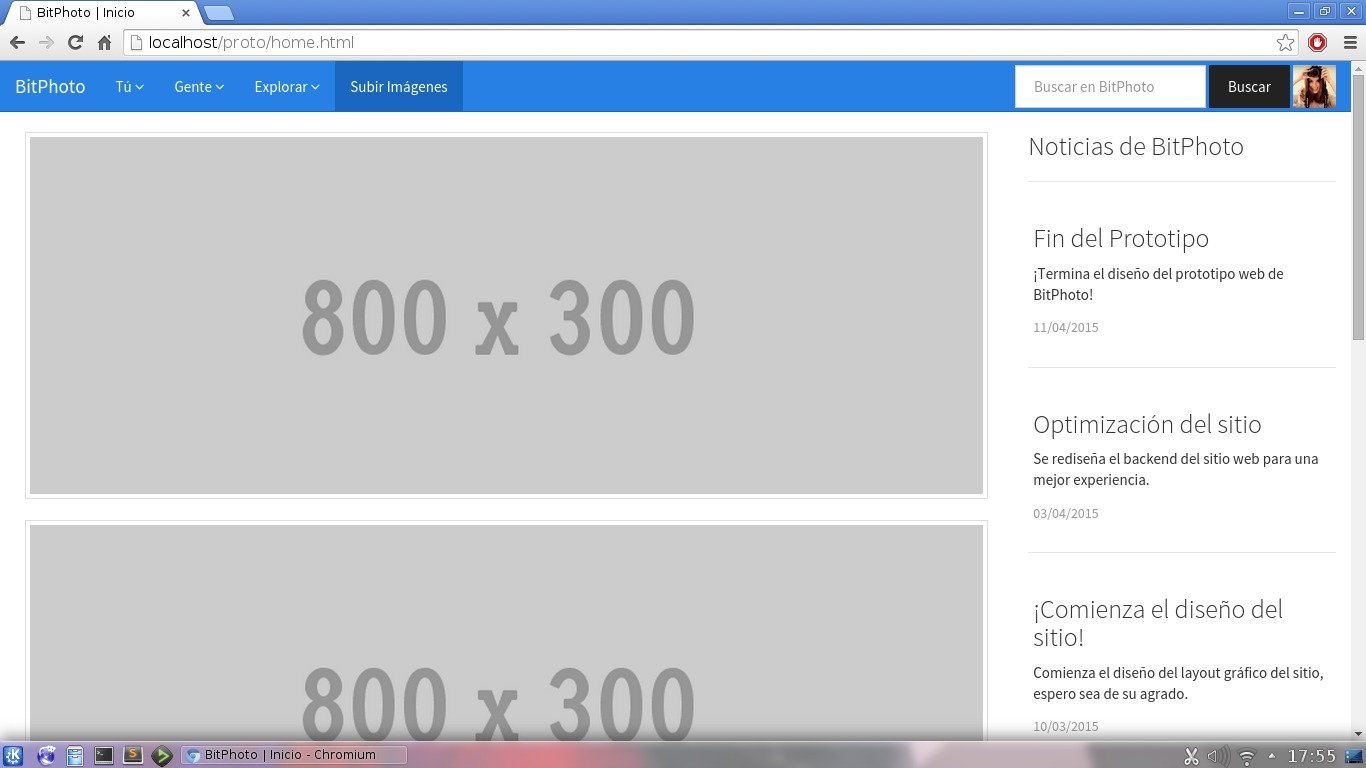
\includegraphics[width=14cm]{proto/04.jpg}
}

Todos los menús y submenús del programa están basados en elementos de Bootstrap.
\figura{Vista Submenú}{
	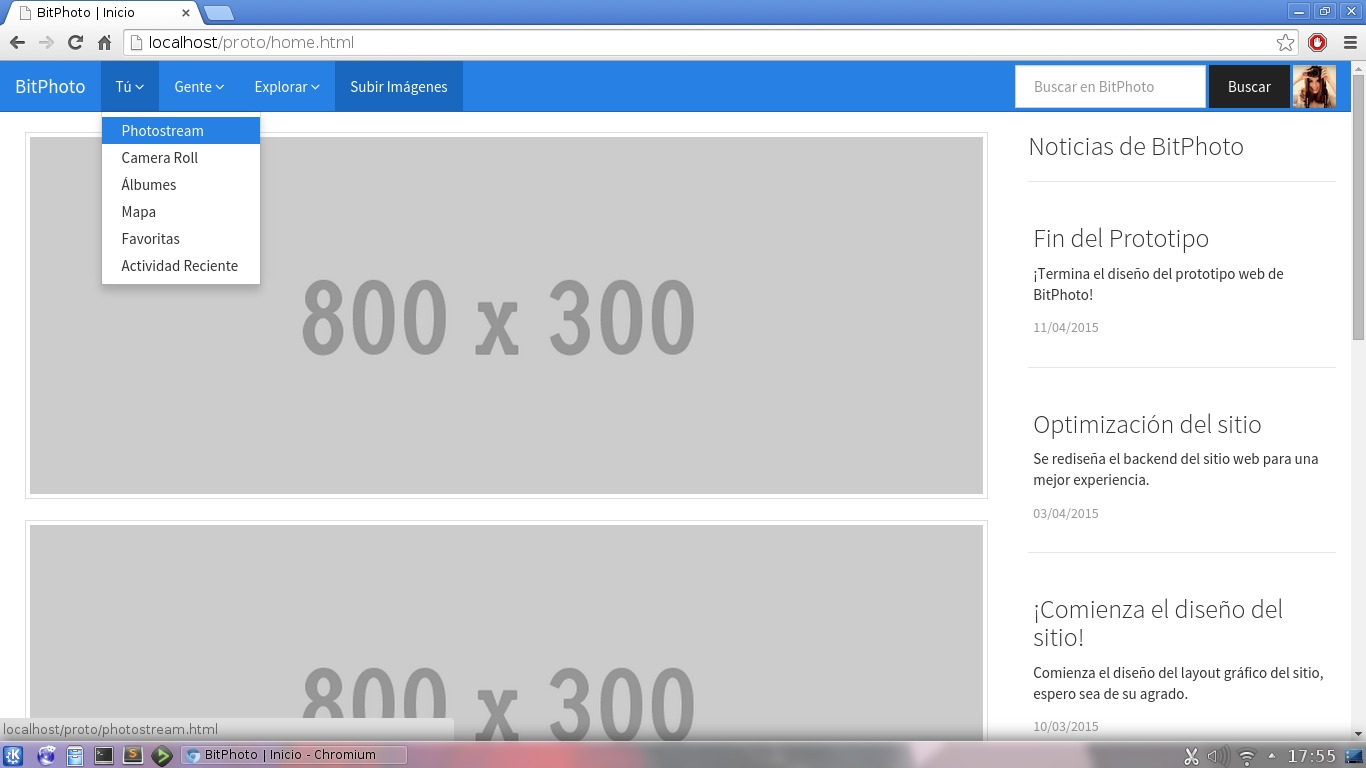
\includegraphics[width=14cm]{proto/05.jpg}
}

\newpage

La vista de Photostream (al igual que la de Album y Favorites), muestra el nombre del usuario, su apodo, su avatar y una galería de imágenes acorde al contenido de la vista seleccionada.
\figura{Vistas Photstream, Álbumes y Favoritas}{
	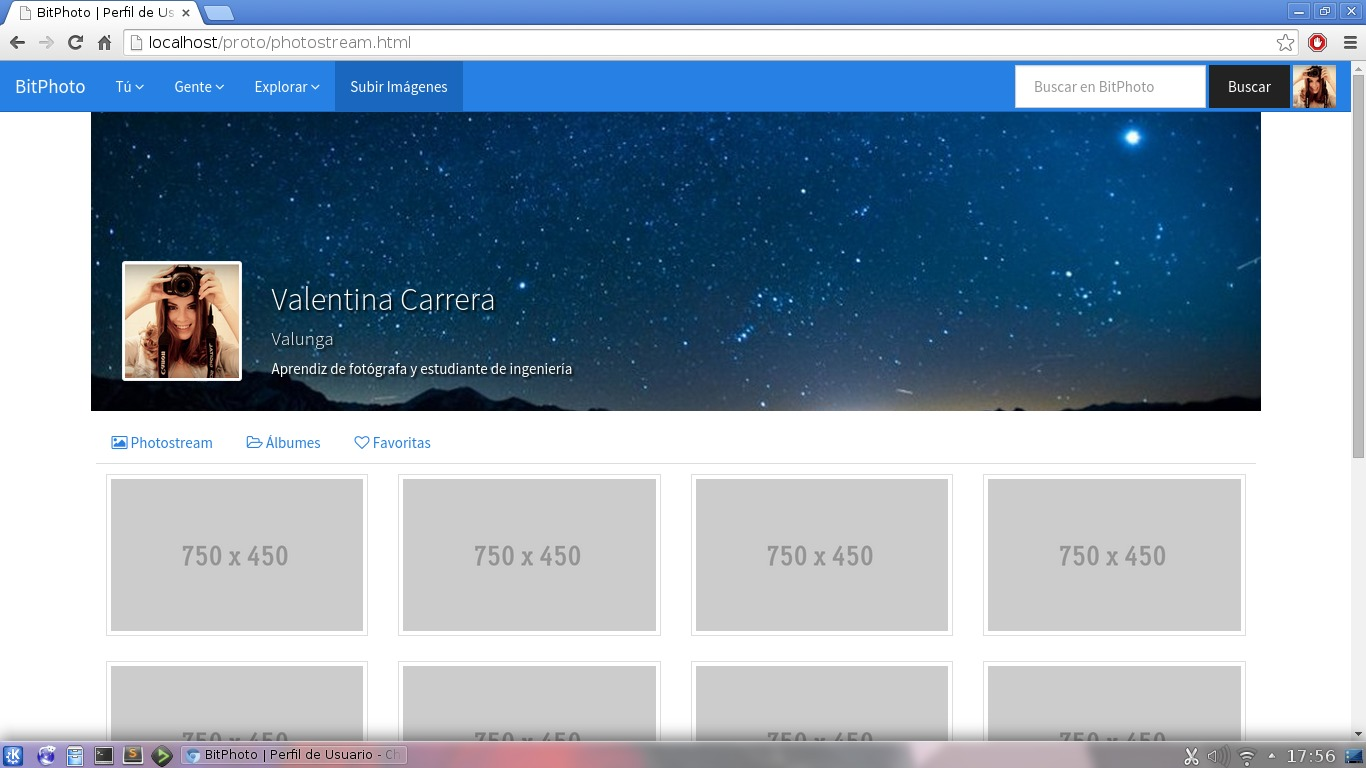
\includegraphics[width=14cm]{proto/06.jpg}
}

La vista Camera Roll permite visualizar las imágenes por intervalos de tiempo. Las imágenes de las vistas serán cargadas a futuro desde la base de datos y serán mostradas con el layout siguiente.
\figura{Vista Camera Roll}{
	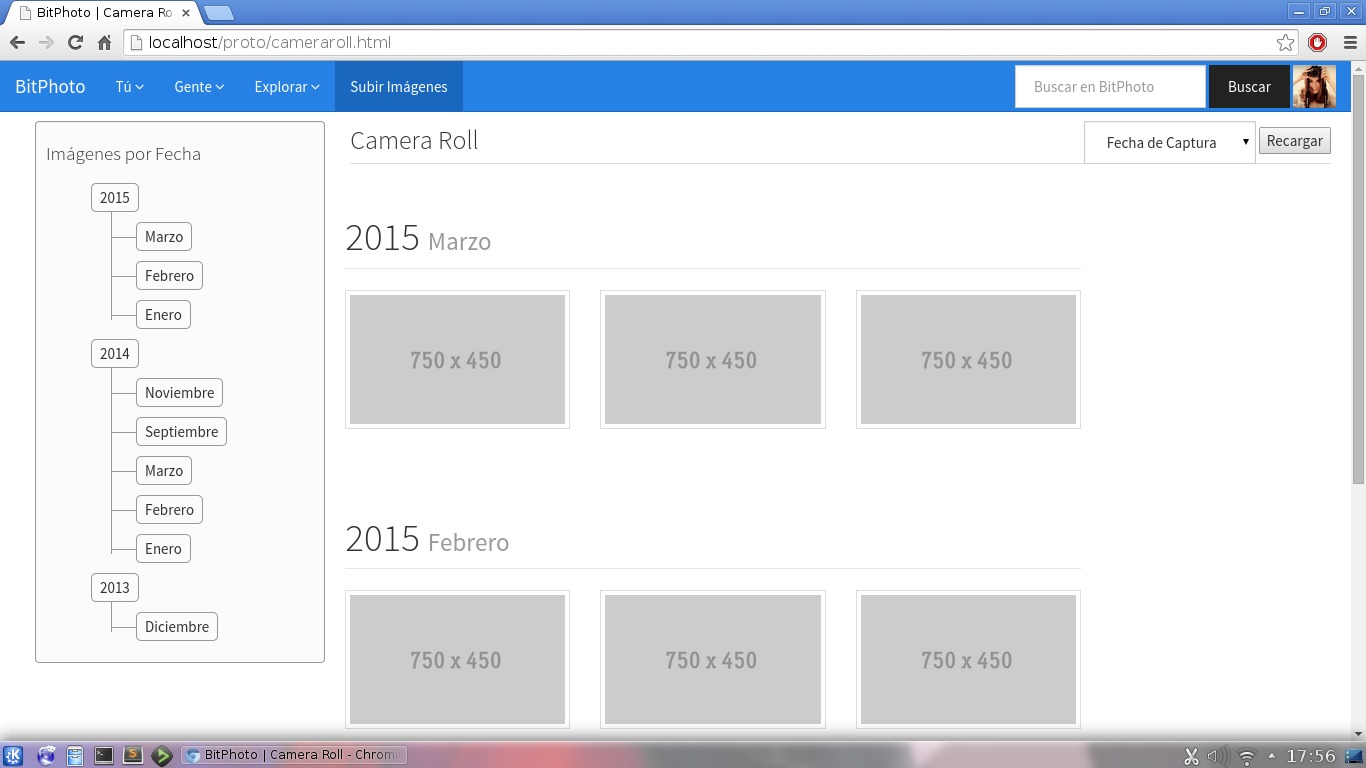
\includegraphics[width=14cm]{proto/07.jpg}
}

\newpage

Las vistas de Mapa no se han implementado en este prototipo, pero se ha dejado el espacio para que sean desarrolladas a futuro.
\figura{Vistas Map y World Map}{
	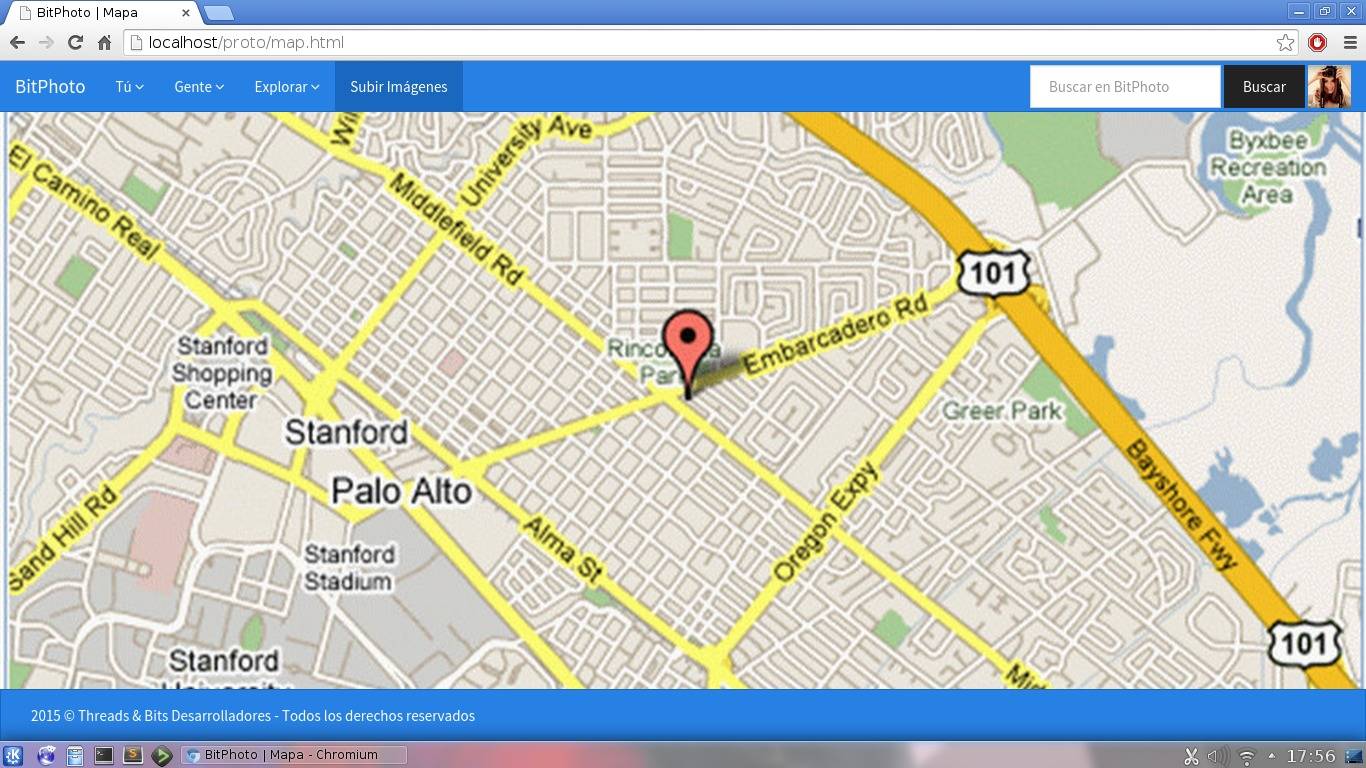
\includegraphics[width=14cm]{proto/08.jpg}
}

La vista de Actividad Reciente muestra las últimas acciones de los seguidos por un usuario, esta vista se elaboró con elementos sencillos para su fácil lectura.
\figura{Vista Recent Activity}{
	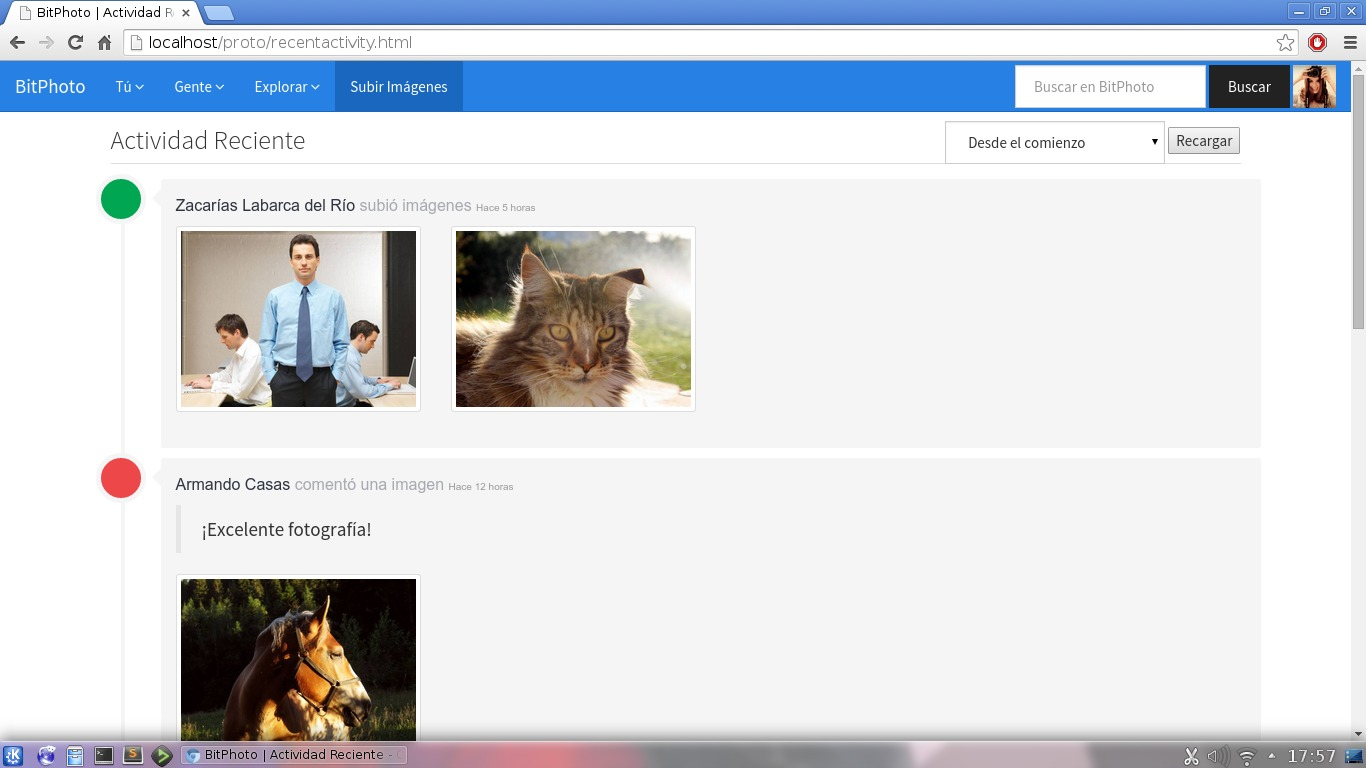
\includegraphics[width=14cm]{proto/09.jpg}
}

\newpage

En la vista Photos from/of se escogió un diseño en grilla sencillo para las imágenes. Nótese que todas las vistas de imágenes del sitio usan clases de diseño adaptativas al tamaño de la pantalla del dispositivo, potenciadas por la tecnología de Bootstrap.
\figura{Vistas Photos From y Photos Of}{
	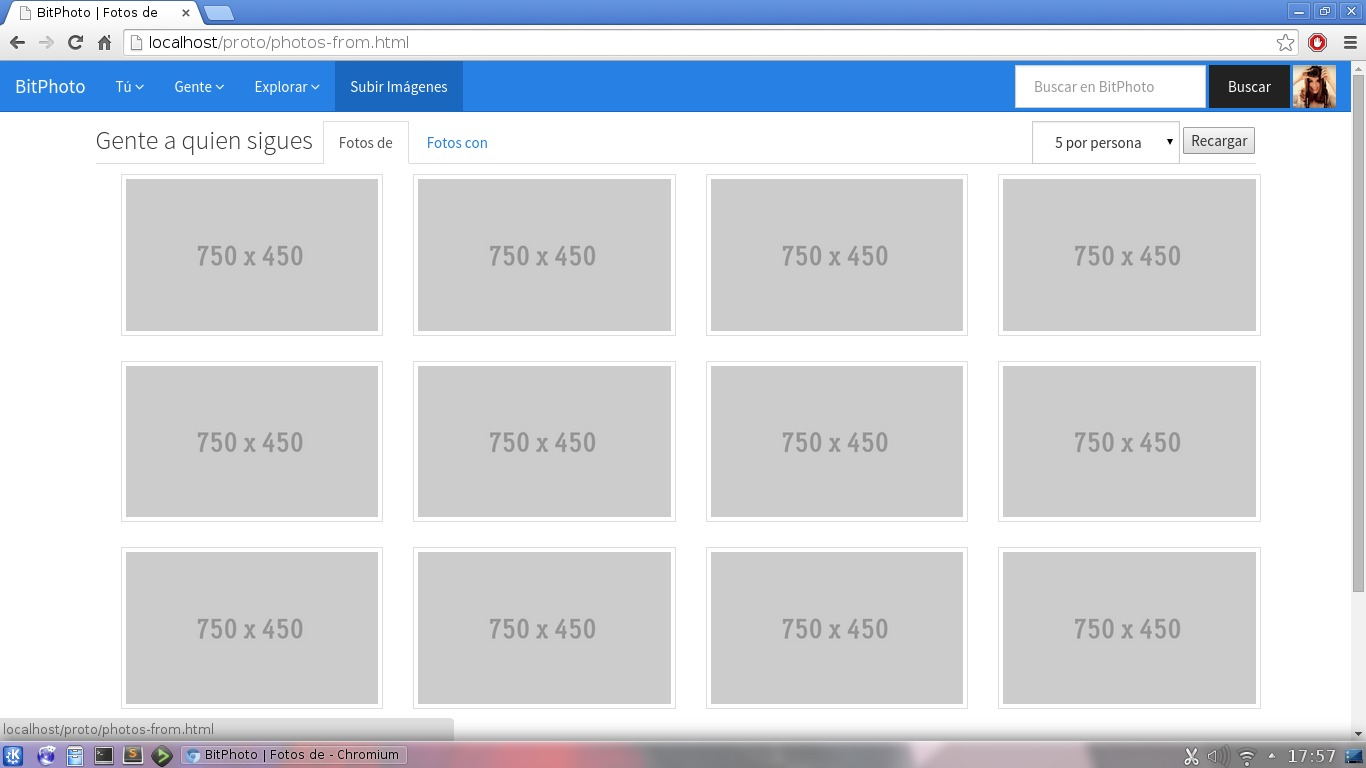
\includegraphics[width=14cm]{proto/10.jpg}
}

Vista de imágenes recientes.
\figura{Vista Recent Photos}{
	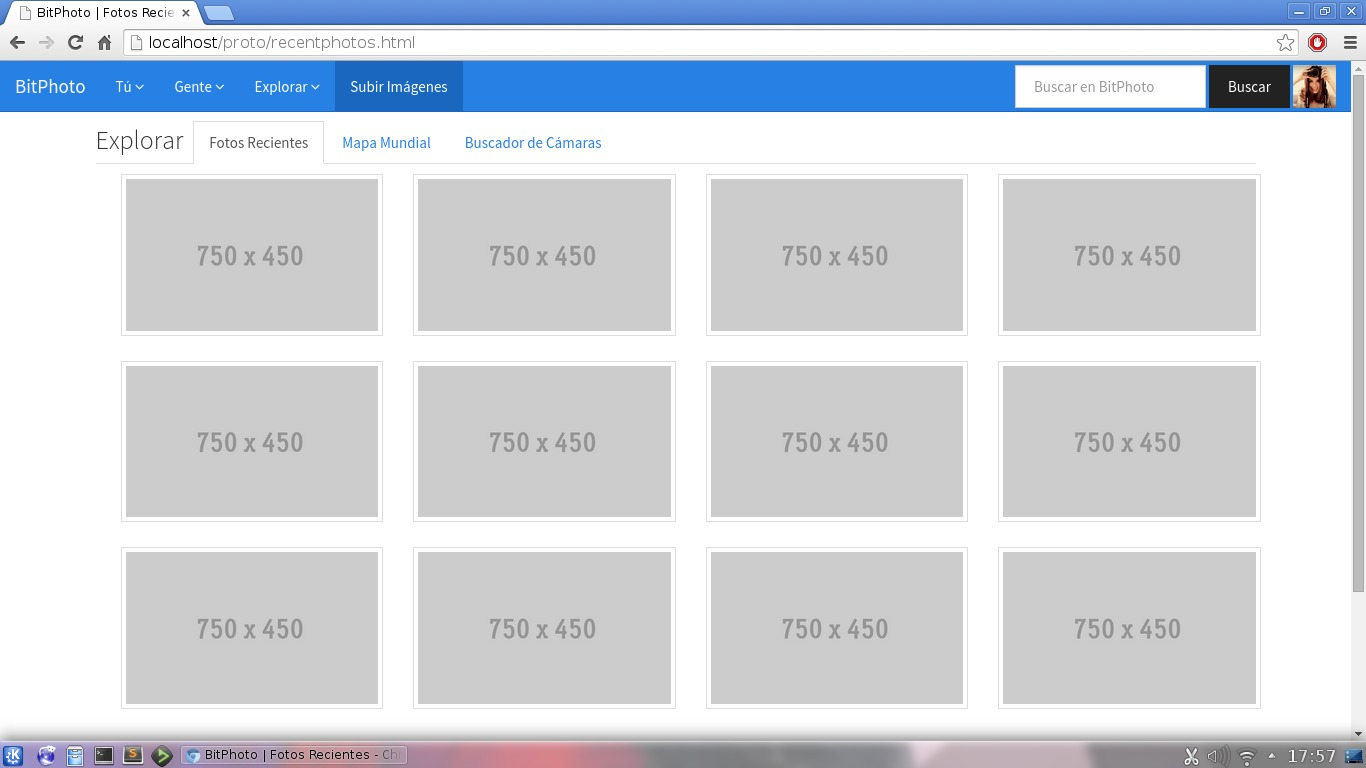
\includegraphics[width=14cm]{proto/11.jpg}
}

\newpage

La vista Camera Finder permite ver las cámaras más usadas del sitio, dichas estadísticas estarán potenciadas por la base de datos.
\figura{Vista Camera Finder}{
	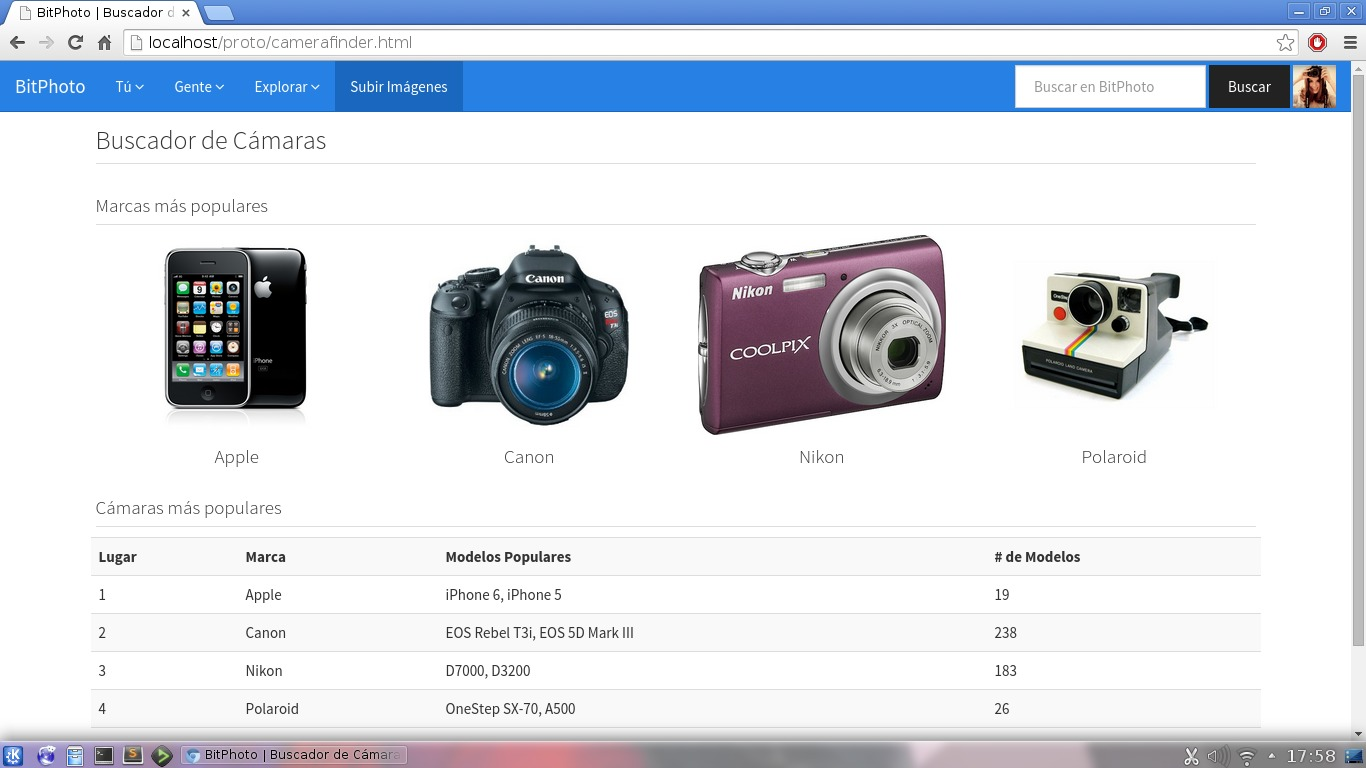
\includegraphics[width=14cm]{proto/12.jpg}
}

Subir imágenes es tarea sencilla en el sitio, el Uploader presenta un diseño claro y estará potenciado por tecnologías JavaScript.
\figura{Vista Upload Photo}{
	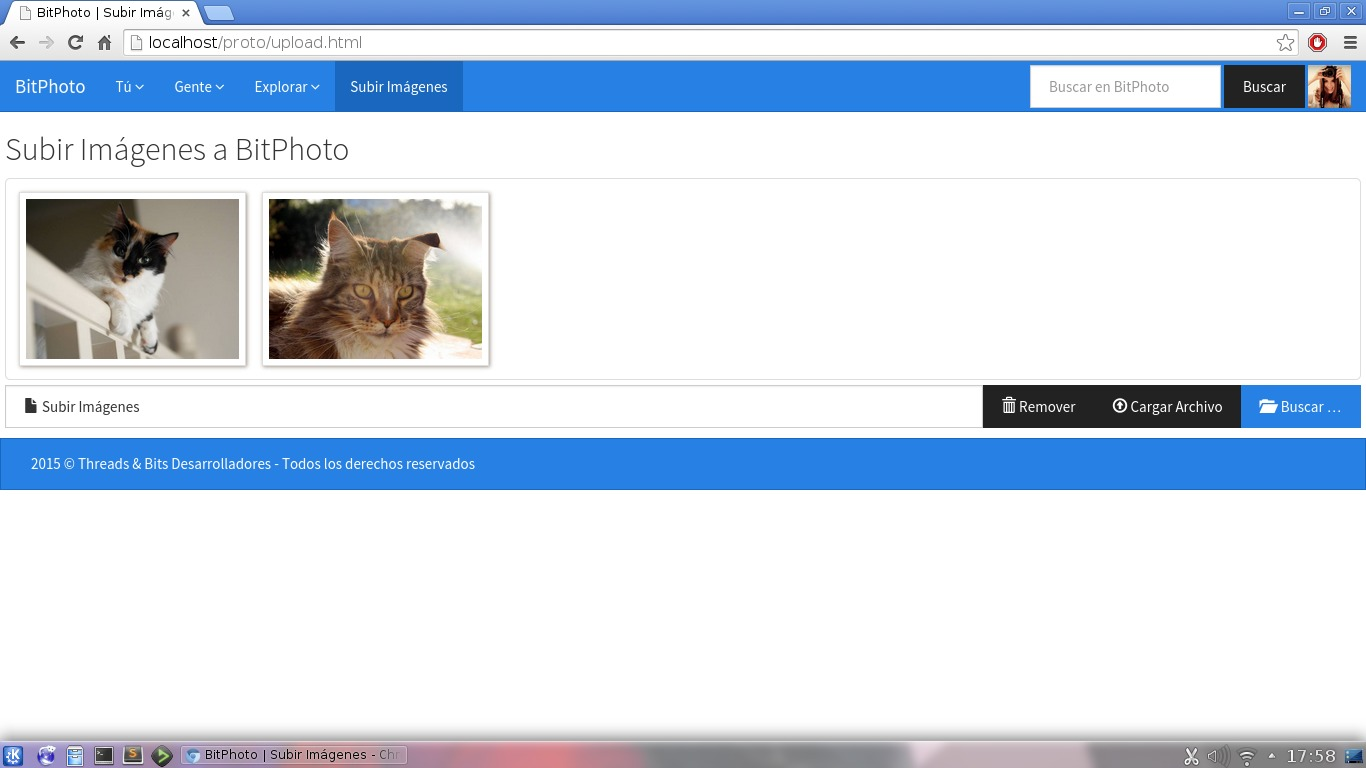
\includegraphics[width=14cm]{proto/13.jpg}
}

\newpage

La búsqueda presenta un diseño similar a los ya vistos en el prototipo, pero agrega tabs selectivos que permiten buscar cualquier foto, fotos propias o de amigos.
\figura{Vista Search}{
	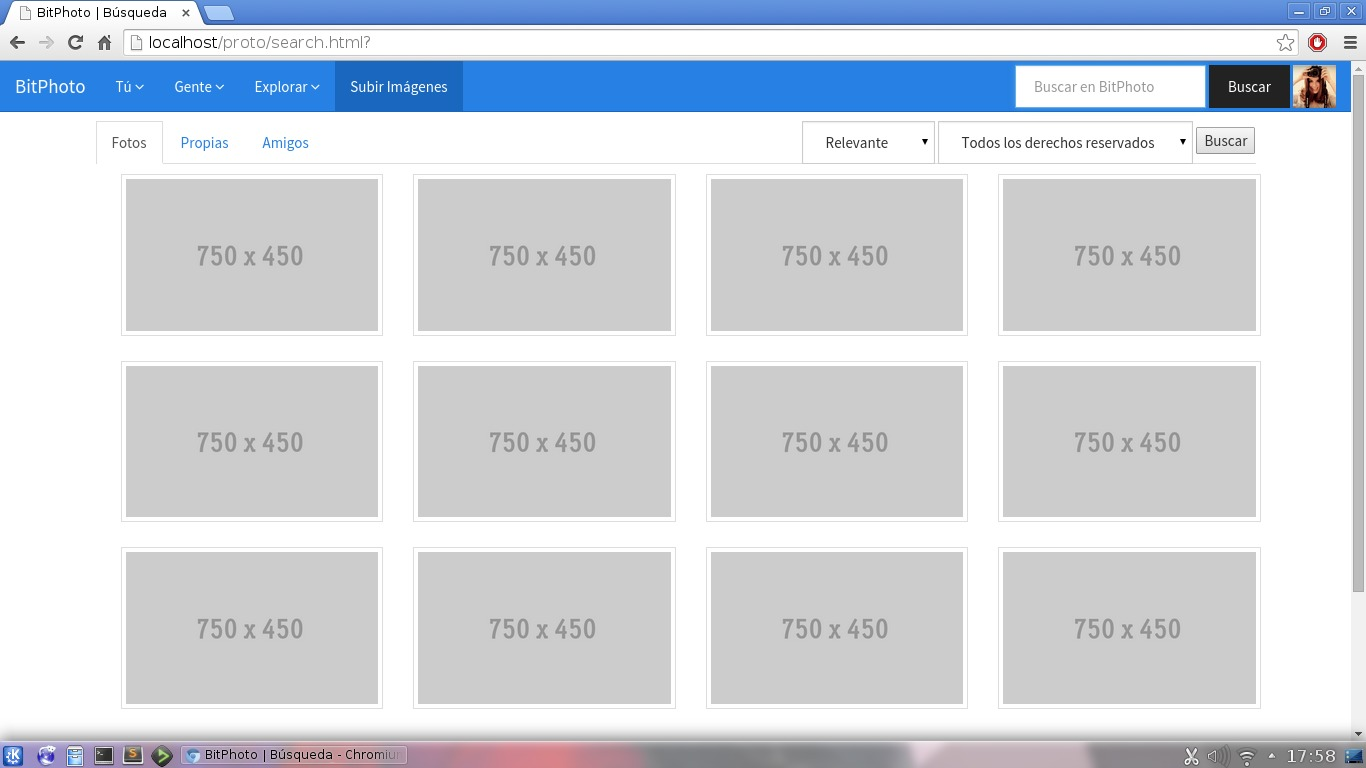
\includegraphics[width=14cm]{proto/14.jpg}
}


%-------------------------------------------------------------------------------------
\capitulo{GESTIÓN DEL PROYECTO.}

\seccion{DEFINICIÓN DE ROLES.}

- \textbf{Elías González Marincovic}: Encargado de la funcionalidad lógica de la aplicación utilizando servicios propios de Java EE, JavaRestfull y encargado de la intercomunicación de los diversos componentes del sistema.\\

- \textbf{Nicolas Rozas Sepúlveda}: Es el especialista en Base de Datos, será el encargado de utilizar las herramientas y administrar la base de datos relacional (distribuir, poblar tablas, etc), utilizando las tecnologías, MySQL y en diseño Sybase PowerDesigner u otras.\\

- \textbf{Daniel Gacitúa Vásquez}: Encargado de la interfaz web que poseerá la aplicación, la cual debe  facilitar las consultas que los usuarios deseen realizar al servidor de aplicaciones mediante una interfaz adecuada, utilizando una presentación correcta para la funcionalidad que se le dará a "BitPhoto". Para esto se utilizará AngularJS, jQuery y HTML5.\\

- \textbf{Gerson Aguirre Pavez}: Encargado de realizar el buscador, parte importante de las vistas que se solicitan, utilizando la herramienta Apache Lucene junto con la aplicación de índices invertidos para la indexación de datos.\\

- \textbf{Max Chacón Villanueva}: Encargado de la aplicación móvil. Estará a cargo de posibilitar el uso de "BitPhoto" en dispositivos Android.\\


Cabe destacar que se asignaron compañeros de apoyo para los diversos roles, quedando la organización de la siguiente manera:

\begin{itemize}
	\item \textbf{Base de Datos}: Encargado Nicolas - Soporte Elías.
	\item \textbf{Aplicación Web}: Encargado Daniel - Soporte Nicolás.
	\item \textbf{Java REST}: Encargado Elías - Soporte Gerson.
	\item \textbf{Aplicación Móvil}: Encargado Max - Soporte Daniel.
	\item \textbf{Buscador}: Encargado Gerson - Soporte Max.
\end{itemize}

También es importante señalar que todos los miembros del Grupo de trabajo estarán encargados de asegurar la calidad del producto (aplicación "BitPhoto"), es decir todos son responsables de la revisión de todos los procesos y tareas que se realicen, además de velar porque se cumplan los resultados que se esperan y que se realice todo de manera correcta.

\newpage

\seccion{DEFINICIÓN DE HERRAMIENTAS.}

A continuación se describe de manera breve y generalizada las tecnologías y herramientas a utilizar para el desarrollo de BitPhoto, para lo cual se han divididoen tres categorías asociadas al sistema a desarrollar, como lo es el Back-End (asociada a la lógica del negocio o lógica de la aplicación), el Front-End (que hace referencia a la parte del sistema que interactúa directamente con el usuario del sistema) y de uso generalizado para el desarrollo del proyecto.  Cabe destacar que las herramientas utilizadas se escogieron con el fin de lograr los requisitos planteados anteriormente.\\

\subseccion{HERRAMIENTAS BACK-END.}

\textbf{Glassfish Server}: Es un servidor de aplicaciones desarrollado por Sun Microsystems, el cual implementa tecnologías definidas para JEE. Es gratuita y de código libre, pero también posee una versión comercial. Posee como servidor base a Sun Java System Application Server de la corporación Oracle. El fin de utilizar Glassfish como servidor de aplicaciones es que permite proporcionar servicios a computadoras clientes, donde los clientes pueden acceder a los datos o conectarse con la parte lógica de la aplicación. Además es compatible con la plataforma JavaEE de esta forma se podrá conectar con JavaEE RESTful.\\

\textbf{MySQL Comunity Edition 5.0+}: Es un sistema que gestiona bases de datos tipo relacional, con capacidad multihilo y multiusuario, desarrollado por Sun Microsystems (MySQL AB), aunque actualmente se desarrolla como software libre, además de poseer una versión comercial. MySQL Comunity Edition es un conjunto de programas que permiten almacenar, modificar y extraer información desde una base de datos, junto con proporcionar herramientas para añadir, borrar, modificar y analizar datos. También cabe destacar que proporciona métodos para mantener la integridad en los datos de la base de datos, controlando el acceso a usuarios, otorgando niveles de permisos para operar sobre la base de datos y recuperar información en caso de ser corrupta mediante una copia de seguridad. Todo lo señalado anteriormente está acompañado y representado mediante una interfaz comoda y facil de utilizar.\\

\textbf{Apache Lucene 4.0+}: Es una API de código abierto, que se agregará como biblioteca al proyecto en Java. Que tiene como fin la búsqueda y recuperacion de informacion, creada por Doug Cutting. Actualmente está apoyado por la fundación de software de Apache y se distribuye bajo la licencia Apache Software License. En este caso se utilizaran sus características de indexado y búsqueda de texto para realizar el buscador de imágenes dentro de BitPhoto. Se basa en el concepto de documentos los cuales poseen determinados campos de texto, permitiendo así trabajar con diferentes formatos de texto.\\

\textbf{Weka 3.5+}: Es una plataforma de software que se caracteriza por el aprendizaje automático y se utiliza frecuentemente en la minería de datos, es una biblioteca escrita en Java y desarrollada por la Universidad de Waikato. Es un software distribuido bajo la licencia GNU GPL. Consiste en una colección de programas con algoritmos de aprendizaje que se encargan de procesar una serie de datos. Estos algoritmos se utilizan para entregar resultados luego de procesar los datos, mediante tareas de clasificación, regresión, asociación, entre otras. Con este conjunto de software se tiene como objetivo crear un analizador de sentimientos, para lo cual se entrenará un modelo con el fin de determinar los sentimientos de los comentarios que realizan los usuarios de BitPhoto, caracterizando estos como positivo, negativo o neutro.\\

\textbf{Netbeans JavaEE 7.0+}: Es un entorno de desarrollo libre, creado principalmente para trabajar con el lenguaje Java. Posee una gran compatibilidad con diferentes tecnologías. Es un producto libre, aunque también existe una versión comercial. Para este proyecto se utilizará para realizar la integración entre las partes de nuestro sistema, conectar la base de datos con la lógica de la aplicación, así también con los módulos respectivos al buscador y clasificador, como también servir la aplicación creada.\\

\subseccion{HERRAMIENTAS FRONT-END.}

\textbf{AngularJS 1.3+}: Es un framework de JavaScript de código abierto, mantenido con el apoyo de google. Tiene como objetivo apoyar la creación de aplicaciones basadas en la capacidad del navegador con un modelo MVC, incluyendo así facilidades para el desarrollo y la prueba del código. El objetivo de utilizar esta herramienta está en desarrollar un esquema de aplicación web basado en rutas, potenciado por el uso de JavaScript y HTML5.\\

\textbf{Bootstrap 3.3+}: Es un framework de diseño web, libre y de código abierto, que contiene una colección de herramientas para la creación de sitios web y aplicaciones web . Contiene código predefinido HTML5 y plantillas CSS, para determinar la forma de los botones, textos, características en la navegación entre otras. Lo utilizaremos también para la creación de la interfaz tanto web de BitPhoto con el fin de agilizar el desarrollo de la interfaz, al mismo tiempo que ésta queda con un diseño adaptativo y homogéneo.\\

\textbf{jQuery 1.x}: Es una biblioteca de JavaScript, creada en un comienzo por John Resing, esta biblioteca permite simplificar la manera de interactuar entre documentos HTML, manejar eventos, desarrollar animaciones, entre otras cosas. Todo esto complementado con la técnica AJAX para la creación de páginas web. Licencia MIT. jQuery otorgará funcionalidades basadas en JavaScript para la creación de BitPhoto, permitiendo lograr grandes resultados en menos tiempo y menos líneas de código.\\

\textbf{HTML5}: Lenguaje de marcado para la creacion de paginas web. Es un lenguaje estándar que sirve de referencia para la elaboración de sitios web. Para este caso permitirá definir una estructura básica para la interfaz de la aplicación y un código para la definición de contenido web como lo son textos, imágenes, videos, entre otros. En estwe caso se utilizará el último estándar de este lenguaje, que es HTML5.\\

\textbf{CSS3}: Hojas de estilo en cascada o CSS, lenguaje utilizado para la definición de plantillas web, para formatos HTML o XML. Permite estandarizar el diseño en la creación de aplicaciones web. La utilización de CSS 3, última versión de CSS, permitirá estilizar uniformemente la apariencia de los elementos de la aplicación.\\

\textbf{JavaScript 1.8+}: Lenguaje de programación interpretado, quiere decir que se ejecuta del lado del navegador. Se caracteriza por ser orientado a objetos, basado en prototipos y se imperativo. Para este proyecto nos permitirá mejorar la interfaz de usuario y generar paginas web dinamicas.\\

\textbf{Android SDK 19}: Sistema Operativo basado en el kernel de Linux, actualmente desarrollado por Google, y utilizado en dispositivos móviles de manera masiva. Para este caso se desarrollará una aplicación compatible con este sistema operativo para que los usuarios de BitPhoto puedan hacer uso de éste a través de sus dispositivos móviles. Para esto se utilizará el SDK versión 19 para compatibilizar la aplicación con todos los dispositivos Android de versión 4.0 en adelante.\\

\subseccion{HERRAMIENTAS USO GENERAL.}

\textbf{Git}: Es un software que permite controlar las versiones, fue diseñado por Linus Torvalds, con el fin de controlar de manera eficiente y confiable las versiones de archivos de código fuente. El repositorio remoto a utilizar será proporcionado por GitHub el cual entrega espacio para desarrollar el proyecto, y conectar éste con los miembros del equipo de trabajo.\\


\textbf{Gradle}: Es una herramienta de automatización de proyecto, se basa en los principios de Apache Ant y Maven. Permite controlar y configurar el proyecto. Utiliza un grafo dirigido para determinar el orden de las tareas que se pueden ejecutar. Para esta entrega se utilizará Gradle para compilar, desplegar, testear y controlar las diferentes dependencias del proyecto.\\

\textbf{JUnit}: Es un conjunto de bibliotecas creadas para la programación, con el fin de realizar pruebas unitarias sobre diversos componentes de la aplicación, en especial las realizadas en Java. Nos permitirá ejecutar las clases creadas en Java, de manera controlada para evaluar el funcionamiento de los métodos implementados. Entonces en función de algún valor de entrada para la prueba se evalúa el valor retornado. si es el esperado o no. También se utlizará para controlar las pruebas de regresión, para que cuando se modifique el código se pueda corroborar si el nuevo código cumple con los requerimientos anteriores.\\

\newpage

\seccion{ORGANIZACIÓN DE REPOSITORIOS GIT.}
    
Para optimizar la creación de código, favorecer la correcta colaboración entre los integrantes y tener un versionamiento ordenado del código, se decide emplear a git como sistema de control de versiones, y usar GitHub como servidor remoto de git.\\

Cada miembro del grupo utiliza una cuenta de GitHub:

\begin{itemize}
	\item \textbf{Gerson Aguirre}: \textsl{https://github.com/GersonAguirre}
	\item \textbf{Max Chacón}: \textsl{https://github.com/nanochacon}
	\item \textbf{Daniel Gacitúa}: \textsl{https://github.com/GaciX}
	\item \textbf{Elías González}: \textsl{https://github.com/Elitos}
	\item \textbf{Nicolás Rozas}: \textsl{https://github.com/NicoRozas}
\end{itemize}

Se ha creado la organización “tbd2015” que aloja todos los repositorios del proyecto: \textsl{https://github.com/tbd2015}.\\

Dentro de la organización, se han creado diferentes repositorios para cada módulo del proyecto:

\begin{itemize}
	\item \textbf{InformesTBD}: Contiene los informes y presentaciones del proyecto. 
	\item \textbf{Prototipo}: Contiene el prototipo gráfico de la Aplicación Web.
	\item \textbf{BitPhoto}: Contiene el módulo principal del proyecto (en JavaEE).
	\item \textbf{BitPhoto-Mobile}: Contiene la aplicación para Android del proyecto.
	\item \textbf{BitPhoto-Search}: Contiene el motor de búsqueda (potenciado por Apache Lucene).
	\item \textbf{BitPhoto-Miner}: Contiene el módulo de análisis de sentimientos (potenciado por Weka).
\end{itemize}

Cada miembro del grupo tendrá acceso a todos los repositorios para fomentar la colaboración. Cabe destacar que con un sistema modular de repositorios dentro de la organización ordena de mejor manera los aportes de cada miembro y ayuda a evitar el entorpecimiento al hacer commits de forma concurrente.

\newpage

\seccion{COMUNICACIÓN, AVANCES Y BURNDOWN.}

En la primera reunión realizada planificamos el Sprint, se determinó que el primer Sprint duraría hasta el 17 de Abril del 2015. Además se acordó las horas de trabajo diarias que se podían dedicar a la realización del proyecto, se estimó que cada integrante del grupo podría dedicar a lo máximo 1.5 hrs al dia para el proyecto. Luego se definieron las tareas para que estas se pudieran realizar en un tiempo cercano al de trabajo diario estimado, luego se estimó el tiempo que se demoraría cada tarea en estar realizada. 

Para la realización de la primera entrega el grupo optó por varios canales de comunicación para manejar las relaciones entre los participantes, por lo tanto se determinaron distintas tecnologías para objetivos específicos, los canales usados para comunicarse entre el grupo fueron los siguientes:

\begin{itemize}
	\item Se creó un grupo en WhatsApp, con el fin de conversar inmediatamente y de forma rápida temas relacionados con el proyecto, principalmente se utilizó para dudas cortas y compartir pequeñas opiniones del proyecto. 
	\item Se creó un grupo en Facebook, para registrar minutas, información relevante y noticias que afecten a todos los integrantes del grupo.
	\item Se creo una carpeta en google drive, para con el fin de compartir documento referentes al informe, presentaciones, etc.  
	\item Se utilizó la aplicación Trello para organizar las partes que se debían realizar en la entrega, además esta aplicación permite organizar las partes del proyecto definiendo las tareas personalmente y los tiempos con los que fueron realizadas cada una de estas.
	\item Para controlar las versiones del informe y los prototipo de las vistas se utilizó la herramienta Git que permite controlar las versiones de estas dos partes del proyecto, esta tecnología se utiliza para archivos de texto plano y para controlar las modificaciones que se le pueden realizar a estos.
\end{itemize}

\newpage

A continuación se presentan las tareas definidas y los tiempos estimados.

\figura{Tareas 1-15}{
	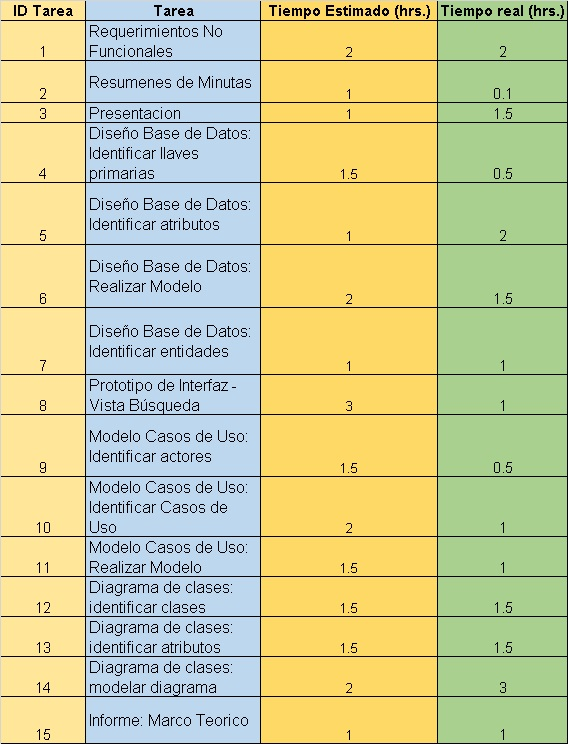
\includegraphics[width=14cm]{burndown/Tareas1.jpg}
}

\figura{Tareas 16-32}{
	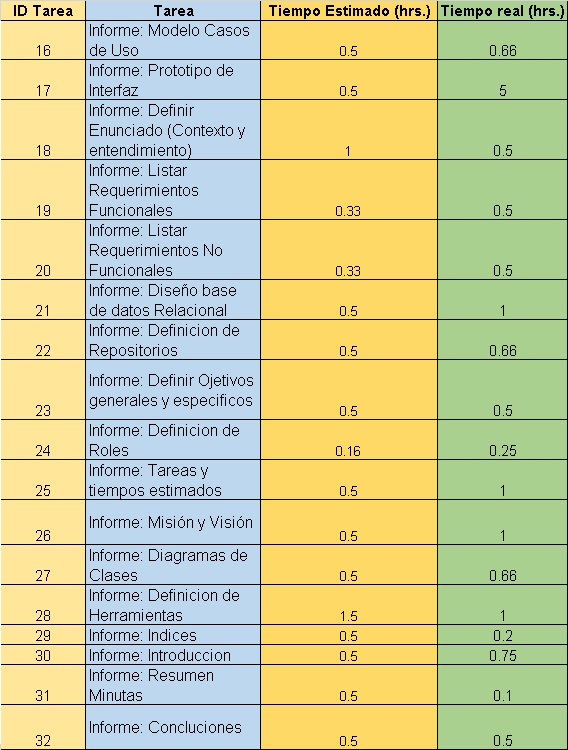
\includegraphics[width=14cm]{burndown/Tareas2.jpg}
}

\figura{Tareas 33-49}{
	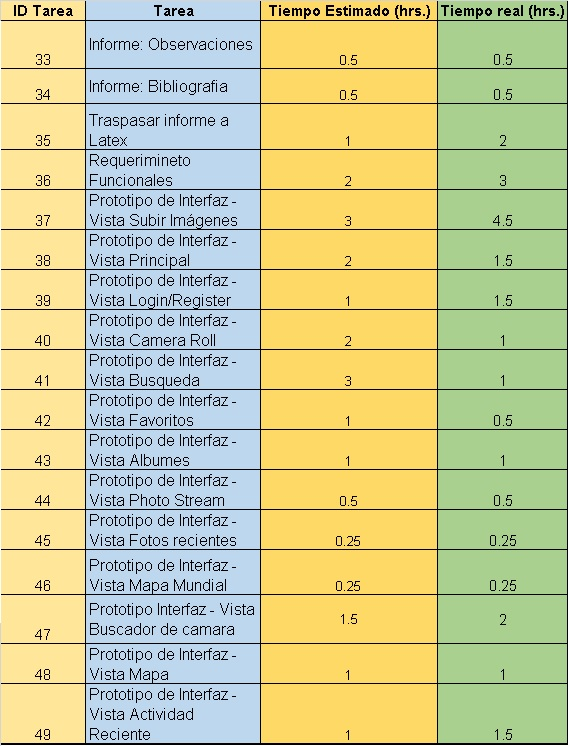
\includegraphics[width=14cm]{burndown/Tareas3.jpg}
}

Ahora la cantidad de horas de trabajos estimadas son 54.32 hrs, Las horas de trabajo real fueron 56.38 , notar que las horas reales trabajadas superaron las horas estimadas en 2,06 hrs aprox, esto quiere decir que las tareas se estimaron correctamente en su mayoría, ya que este margen de error fue relativamente bajo. Tiempo promedio por tarea fue de 1.11 hrs. Otros datos que se obtiene al analizar lo anterior son:

\begin{itemize}
	\item Estimación Trabajo Diario Grupo: 7.5 
	\item Horas Disponibles en Sprint por cada integrante: 37.5 
	\item Horas Disponibles  en Sprint del Grupo: 187.5 
	\item Trabajo por dia promedio ideal 2.59 
\end{itemize}

Cabe señalar que si se trabajara de manera ideal, sobraría  tiempo equivalente a 187.5 hrs - 54.32 hrs = 133.18 hrs . Al pasar una semana se creyó que era necesario definir los roles de cada miembro del grupo para comenzar a trabajar o informarse desde ahora sobre el área en particular designada.

A continuación se presentan los gráficos BurnDown y BurnUP con el fin de señalar la forma en que se trabajó a lo largo del Sprint:

\figura{Gráfico de Burndown/Burnup}{
	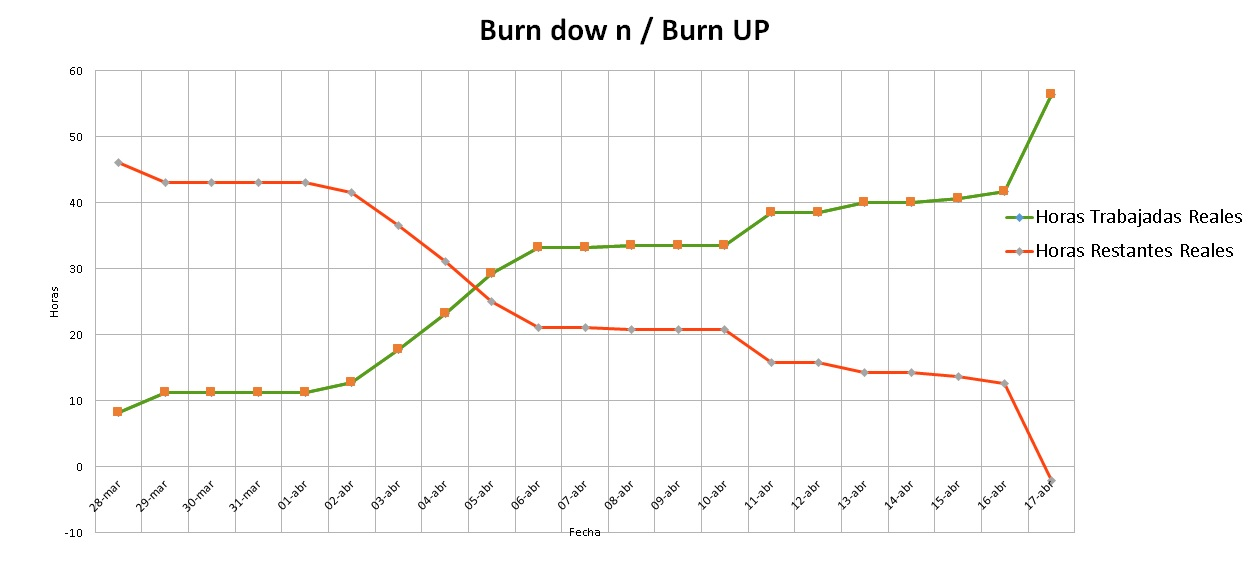
\includegraphics[width=14cm]{burndown/burndown2.jpg}
}

Como se aprecia en la imagen, se observa que en determinados periodos se trabajo una mayor cantidad, si bien alcanzamos a realizar la mitad del trabajo estimado a la fecha 5 de Abril, luego se disminuyó el trabajo realizado por dia a una frecuencia menor, en los últimos días se aumentó la frecuencia de trabajo para el los días antes de la entrega del informe. Otra cosa que se aprecia es que desde el primer dia en el que se definió el SPRINT se comenzó a trabajar por eso la grafica no comienza desde cero.



%-------------------------------------------------------------------------------------
\capitulo{OBSERVACIONES.}

Se añaden las observaciones realizadas al trabajo durante la 1º Presentación del Proyecto:

\tabla{Observación OBS1}{
	\begin{tabular}[c]{|p{4cm}|p{11cm}|}
		\hline
		Número Observación & OBS1\\ \hline
		Detalle Observación & El RF41 es un requisito funcional del browser no de la aplicacion.\\ \hline
		Acción a Realizar & Se elimina el RF41 (El usuario puede mantener sus sesión iniciada mediante la opción “Recordar sesión”).\\ \hline
		Justificación & Este requisito es del navegador web, no de la aplicación en si.\\ \hline
		Página del Informe & 22\\ \hline
	\end{tabular}
}

\tabla{Observación OBS2}{
	\begin{tabular}[c]{|p{4cm}|p{11cm}|}
		\hline
		Número Observación & OBS2\\ \hline
		Detalle Observación & El RNF4 tiene que especificar el estandar de los datos geo-espaciales.\\ \hline
		Acción a Realizar & Redactar nuevamente en el requisito no funcional numero 4.\\ \hline
		Justificación & En el requisito se debe especificar el formato estandar que utilizan los datos geo-espaciales.\\ \hline
		Página del Informe & 23\\ \hline
	\end{tabular}
}

\tabla{Observación OBS3}{
	\begin{tabular}[c]{|p{4cm}|p{11cm}|}
		\hline
		Número Observación & OBS3\\ \hline
		Detalle Observación & Explicacion de los canales de comunicacion.\\ \hline
		Acción a Realizar & Redactar un texto que muestre los canales de comunicacion utilizados en la realizacion de la entrega.\\ \hline
		Justificación & Por proósitos de documetnación, en el informe se deben detallar los canales que utilizaron los participantes.\\ \hline
		Página del Informe & 52\\ \hline
	\end{tabular}
}

\newpage

\tabla{Observación OBS4}{
	\begin{tabular}[c]{|p{4cm}|p{11cm}|}
		\hline
		Número Observación & OBS4\\ \hline
		Detalle Observación & En el grafico de Burndown mostrar solo curvas reales.\\ \hline
		Acción a Realizar & Cambiar el grafico de burdown con otro con solo las curvas reales del trabajo.\\ \hline
		Justificación & Muchas lineas confunden al que observa el grafico, este deberia ser mas simple y solo mostrar las curvas reales.\\ \hline
		Página del Informe & 56\\ \hline
	\end{tabular}
}

%-------------------------------------------------------------------------------------
\capitulonn{CONCLUSIONES.}

Luego de finalizar la primera entrega del proyecto correspondiente a la ingeniería de requerimientos, se ha concluido en dos perspectivas que se estiman  adecuadas a la hora de realizar futuros trabajos, perspectiva a nivel de la ingeniería de requerimientos y la perspectiva de trabajo en equipo.
Con respecto a la ingeniería de requerimientos y ciertos aspectos utilizados a la hora de realizar la entrega, se puede decir que las herramientas utilizadas y mencionadas con anterioridad en el informe, han facilitado muchos aspectos, agregando además que han ampliado la perspectiva del proyecto, logrando así entender en profundidad cómo funciona el sistema a crear,  cuales son estas funcionalidades y cómo se pueden crear a futuro. 
Es por esto que se puede decir que esta etapa en la ingeniería de software es fundamental a la hora de iniciar el proyecto.
En la otra perspectiva a nivel del trabajo en equipo, se puede concluir que se ha logrado una gran comunicación entre cada uno de los integrantes del grupo y una buena organización debido a esto mismo, en conjunto con las herramientas de carácter social se ha logrado un gran avance en relación al trabajo en equipo. 
Finalmente como conclusión general se puede decir que se ha trabajado de manera íntegra cumpliendo a cabalidad los objetivos específicos tanto como generales que se han planteado.


%-------------------------------------------------------------------------------------

\capitulonn{BIBLIOGRAFÍA.}

\begin{itemize}
	\item Glassfish: https://glassfish.java.net/es/
	\item MySQL: http://www.mysql.com/
	\item Weka: http://www.cs.waikato.ac.nz/ml/weka/
	\item Bibliografia: https://lucene.apache.org/
	\item Netbeans: https://netbeans.org/
	\item AngularJS : https://angularjs.org/
	\item Bootstrap: http://getbootstrap.com/
	\item JQuery: https://jquery.com/
	\item CSS3: http://www.css3.info/
	\item HTML5: http://www.w3schools.com/html/html5\_intro.asp
	\item JavaScript: http://www.w3schools.com/js/
	\item Android: https://www.android.com/
	\item Git: http://git-scm.com/
	\item Gradle: https://gradle.org/
	\item JUnit : http://junit.org/
	\item Diagrama de clases: http://users.dcc.uchile.cl/~psalinas/uml/modelo.html
	\item Mision y Vision: http://es.slideshare.net/ponceguillermo71/concepto-de-mision-y-vision
\end{itemize}

\end{document}
